\documentclass[11pt]{article}

    \usepackage[breakable]{tcolorbox}
    \usepackage{parskip} % Stop auto-indenting (to mimic markdown behaviour)
    
    \usepackage{iftex}
    \ifPDFTeX
    	\usepackage[T1]{fontenc}
    	\usepackage{mathpazo}
    \else
    	\usepackage{fontspec}
    \fi

    % Basic figure setup, for now with no caption control since it's done
    % automatically by Pandoc (which extracts ![](path) syntax from Markdown).
    \usepackage{graphicx}
    % Maintain compatibility with old templates. Remove in nbconvert 6.0
    \let\Oldincludegraphics\includegraphics
    % Ensure that by default, figures have no caption (until we provide a
    % proper Figure object with a Caption API and a way to capture that
    % in the conversion process - todo).
    \usepackage{caption}
    \DeclareCaptionFormat{nocaption}{}
    \captionsetup{format=nocaption,aboveskip=0pt,belowskip=0pt}

    \usepackage{float}
    \floatplacement{figure}{H} % forces figures to be placed at the correct location
    \usepackage{xcolor} % Allow colors to be defined
    \usepackage{enumerate} % Needed for markdown enumerations to work
    \usepackage{geometry} % Used to adjust the document margins
    \usepackage{amsmath} % Equations
    \usepackage{amssymb} % Equations
    \usepackage{textcomp} % defines textquotesingle
    % Hack from http://tex.stackexchange.com/a/47451/13684:
    \AtBeginDocument{%
        \def\PYZsq{\textquotesingle}% Upright quotes in Pygmentized code
    }
    \usepackage{upquote} % Upright quotes for verbatim code
    \usepackage{eurosym} % defines \euro
    \usepackage[mathletters]{ucs} % Extended unicode (utf-8) support
    \usepackage{fancyvrb} % verbatim replacement that allows latex
    \usepackage{grffile} % extends the file name processing of package graphics 
                         % to support a larger range
    \makeatletter % fix for old versions of grffile with XeLaTeX
    \@ifpackagelater{grffile}{2019/11/01}
    {
      % Do nothing on new versions
    }
    {
      \def\Gread@@xetex#1{%
        \IfFileExists{"\Gin@base".bb}%
        {\Gread@eps{\Gin@base.bb}}%
        {\Gread@@xetex@aux#1}%
      }
    }
    \makeatother
    \usepackage[Export]{adjustbox} % Used to constrain images to a maximum size
    \adjustboxset{max size={0.9\linewidth}{0.9\paperheight}}

    % The hyperref package gives us a pdf with properly built
    % internal navigation ('pdf bookmarks' for the table of contents,
    % internal cross-reference links, web links for URLs, etc.)
    \usepackage{hyperref}
    % The default LaTeX title has an obnoxious amount of whitespace. By default,
    % titling removes some of it. It also provides customization options.
    \usepackage{titling}
    \usepackage{longtable} % longtable support required by pandoc >1.10
    \usepackage{booktabs}  % table support for pandoc > 1.12.2
    \usepackage[inline]{enumitem} % IRkernel/repr support (it uses the enumerate* environment)
    \usepackage[normalem]{ulem} % ulem is needed to support strikethroughs (\sout)
                                % normalem makes italics be italics, not underlines
    \usepackage{mathrsfs}
    
    
    \usepackage{pgfplots}
    \pgfplotsset{compat=1.15}
    \usepackage{mathrsfs}
    \usetikzlibrary{arrows}

    
    % Colors for the hyperref package
    \definecolor{urlcolor}{rgb}{0,.145,.698}
    \definecolor{linkcolor}{rgb}{.71,0.21,0.01}
    \definecolor{citecolor}{rgb}{.12,.54,.11}

    % ANSI colors
    \definecolor{ansi-black}{HTML}{3E424D}
    \definecolor{ansi-black-intense}{HTML}{282C36}
    \definecolor{ansi-red}{HTML}{E75C58}
    \definecolor{ansi-red-intense}{HTML}{B22B31}
    \definecolor{ansi-green}{HTML}{00A250}
    \definecolor{ansi-green-intense}{HTML}{007427}
    \definecolor{ansi-yellow}{HTML}{DDB62B}
    \definecolor{ansi-yellow-intense}{HTML}{B27D12}
    \definecolor{ansi-blue}{HTML}{208FFB}
    \definecolor{ansi-blue-intense}{HTML}{0065CA}
    \definecolor{ansi-magenta}{HTML}{D160C4}
    \definecolor{ansi-magenta-intense}{HTML}{A03196}
    \definecolor{ansi-cyan}{HTML}{60C6C8}
    \definecolor{ansi-cyan-intense}{HTML}{258F8F}
    \definecolor{ansi-white}{HTML}{C5C1B4}
    \definecolor{ansi-white-intense}{HTML}{A1A6B2}
    \definecolor{ansi-default-inverse-fg}{HTML}{FFFFFF}
    \definecolor{ansi-default-inverse-bg}{HTML}{000000}
    
    \definecolor{fuqqzz}{rgb}{0.9568627450980393,0,0.6}
    \definecolor{ccqqqq}{rgb}{0.8,0,0}
    \definecolor{qqqqff}{rgb}{0,0,1}
    \definecolor{ududff}{rgb}{0.30196078431372547,0.30196078431372547,1}
    \definecolor{zzttff}{rgb}{0.6,0.2,1}
    \definecolor{zzttqq}{rgb}{0.6,0.2,0}
    \definecolor{uuuuuu}{rgb}{0.26666666666666666,0.26666666666666666,0.26666666666666666}
    \definecolor{xdxdff}{rgb}{0.49019607843137253,0.49019607843137253,1}
    \definecolor{cqcqcq}{rgb}{0.7529411764705882,0.7529411764705882,0.7529411764705882}

    % common color for the border for error outputs.
    \definecolor{outerrorbackground}{HTML}{FFDFDF}

    % commands and environments needed by pandoc snippets
    % extracted from the output of `pandoc -s`
    \providecommand{\tightlist}{%
      \setlength{\itemsep}{0pt}\setlength{\parskip}{0pt}}
    \DefineVerbatimEnvironment{Highlighting}{Verbatim}{commandchars=\\\{\}}
    % Add ',fontsize=\small' for more characters per line
    \newenvironment{Shaded}{}{}
    \newcommand{\KeywordTok}[1]{\textcolor[rgb]{0.00,0.44,0.13}{\textbf{{#1}}}}
    \newcommand{\DataTypeTok}[1]{\textcolor[rgb]{0.56,0.13,0.00}{{#1}}}
    \newcommand{\DecValTok}[1]{\textcolor[rgb]{0.25,0.63,0.44}{{#1}}}
    \newcommand{\BaseNTok}[1]{\textcolor[rgb]{0.25,0.63,0.44}{{#1}}}
    \newcommand{\FloatTok}[1]{\textcolor[rgb]{0.25,0.63,0.44}{{#1}}}
    \newcommand{\CharTok}[1]{\textcolor[rgb]{0.25,0.44,0.63}{{#1}}}
    \newcommand{\StringTok}[1]{\textcolor[rgb]{0.25,0.44,0.63}{{#1}}}
    \newcommand{\CommentTok}[1]{\textcolor[rgb]{0.38,0.63,0.69}{\textit{{#1}}}}
    \newcommand{\OtherTok}[1]{\textcolor[rgb]{0.00,0.44,0.13}{{#1}}}
    \newcommand{\AlertTok}[1]{\textcolor[rgb]{1.00,0.00,0.00}{\textbf{{#1}}}}
    \newcommand{\FunctionTok}[1]{\textcolor[rgb]{0.02,0.16,0.49}{{#1}}}
    \newcommand{\RegionMarkerTok}[1]{{#1}}
    \newcommand{\ErrorTok}[1]{\textcolor[rgb]{1.00,0.00,0.00}{\textbf{{#1}}}}
    \newcommand{\NormalTok}[1]{{#1}}
    
    % Additional commands for more recent versions of Pandoc
    \newcommand{\ConstantTok}[1]{\textcolor[rgb]{0.53,0.00,0.00}{{#1}}}
    \newcommand{\SpecialCharTok}[1]{\textcolor[rgb]{0.25,0.44,0.63}{{#1}}}
    \newcommand{\VerbatimStringTok}[1]{\textcolor[rgb]{0.25,0.44,0.63}{{#1}}}
    \newcommand{\SpecialStringTok}[1]{\textcolor[rgb]{0.73,0.40,0.53}{{#1}}}
    \newcommand{\ImportTok}[1]{{#1}}
    \newcommand{\DocumentationTok}[1]{\textcolor[rgb]{0.73,0.13,0.13}{\textit{{#1}}}}
    \newcommand{\AnnotationTok}[1]{\textcolor[rgb]{0.38,0.63,0.69}{\textbf{\textit{{#1}}}}}
    \newcommand{\CommentVarTok}[1]{\textcolor[rgb]{0.38,0.63,0.69}{\textbf{\textit{{#1}}}}}
    \newcommand{\VariableTok}[1]{\textcolor[rgb]{0.10,0.09,0.49}{{#1}}}
    \newcommand{\ControlFlowTok}[1]{\textcolor[rgb]{0.00,0.44,0.13}{\textbf{{#1}}}}
    \newcommand{\OperatorTok}[1]{\textcolor[rgb]{0.40,0.40,0.40}{{#1}}}
    \newcommand{\BuiltInTok}[1]{{#1}}
    \newcommand{\ExtensionTok}[1]{{#1}}
    \newcommand{\PreprocessorTok}[1]{\textcolor[rgb]{0.74,0.48,0.00}{{#1}}}
    \newcommand{\AttributeTok}[1]{\textcolor[rgb]{0.49,0.56,0.16}{{#1}}}
    \newcommand{\InformationTok}[1]{\textcolor[rgb]{0.38,0.63,0.69}{\textbf{\textit{{#1}}}}}
    \newcommand{\WarningTok}[1]{\textcolor[rgb]{0.38,0.63,0.69}{\textbf{\textit{{#1}}}}}
    
    
    % Define a nice break command that doesn't care if a line doesn't already
    % exist.
    \def\br{\hspace*{\fill} \\* }
    % Math Jax compatibility definitions
    \def\gt{>}
    \def\lt{<}
    \let\Oldtex\TeX
    \let\Oldlatex\LaTeX
    \renewcommand{\TeX}{\textrm{\Oldtex}}
    \renewcommand{\LaTeX}{\textrm{\Oldlatex}}
    % Document parameters
    % Document title
    \title{TCP2\_LatticePoints\_WeightMultiplicities}
    
    
    
    
    
% Pygments definitions
\makeatletter
\def\PY@reset{\let\PY@it=\relax \let\PY@bf=\relax%
    \let\PY@ul=\relax \let\PY@tc=\relax%
    \let\PY@bc=\relax \let\PY@ff=\relax}
\def\PY@tok#1{\csname PY@tok@#1\endcsname}
\def\PY@toks#1+{\ifx\relax#1\empty\else%
    \PY@tok{#1}\expandafter\PY@toks\fi}
\def\PY@do#1{\PY@bc{\PY@tc{\PY@ul{%
    \PY@it{\PY@bf{\PY@ff{#1}}}}}}}
\def\PY#1#2{\PY@reset\PY@toks#1+\relax+\PY@do{#2}}

\expandafter\def\csname PY@tok@w\endcsname{\def\PY@tc##1{\textcolor[rgb]{0.73,0.73,0.73}{##1}}}
\expandafter\def\csname PY@tok@c\endcsname{\let\PY@it=\textit\def\PY@tc##1{\textcolor[rgb]{0.25,0.50,0.50}{##1}}}
\expandafter\def\csname PY@tok@cp\endcsname{\def\PY@tc##1{\textcolor[rgb]{0.74,0.48,0.00}{##1}}}
\expandafter\def\csname PY@tok@k\endcsname{\let\PY@bf=\textbf\def\PY@tc##1{\textcolor[rgb]{0.00,0.50,0.00}{##1}}}
\expandafter\def\csname PY@tok@kp\endcsname{\def\PY@tc##1{\textcolor[rgb]{0.00,0.50,0.00}{##1}}}
\expandafter\def\csname PY@tok@kt\endcsname{\def\PY@tc##1{\textcolor[rgb]{0.69,0.00,0.25}{##1}}}
\expandafter\def\csname PY@tok@o\endcsname{\def\PY@tc##1{\textcolor[rgb]{0.40,0.40,0.40}{##1}}}
\expandafter\def\csname PY@tok@ow\endcsname{\let\PY@bf=\textbf\def\PY@tc##1{\textcolor[rgb]{0.67,0.13,1.00}{##1}}}
\expandafter\def\csname PY@tok@nb\endcsname{\def\PY@tc##1{\textcolor[rgb]{0.00,0.50,0.00}{##1}}}
\expandafter\def\csname PY@tok@nf\endcsname{\def\PY@tc##1{\textcolor[rgb]{0.00,0.00,1.00}{##1}}}
\expandafter\def\csname PY@tok@nc\endcsname{\let\PY@bf=\textbf\def\PY@tc##1{\textcolor[rgb]{0.00,0.00,1.00}{##1}}}
\expandafter\def\csname PY@tok@nn\endcsname{\let\PY@bf=\textbf\def\PY@tc##1{\textcolor[rgb]{0.00,0.00,1.00}{##1}}}
\expandafter\def\csname PY@tok@ne\endcsname{\let\PY@bf=\textbf\def\PY@tc##1{\textcolor[rgb]{0.82,0.25,0.23}{##1}}}
\expandafter\def\csname PY@tok@nv\endcsname{\def\PY@tc##1{\textcolor[rgb]{0.10,0.09,0.49}{##1}}}
\expandafter\def\csname PY@tok@no\endcsname{\def\PY@tc##1{\textcolor[rgb]{0.53,0.00,0.00}{##1}}}
\expandafter\def\csname PY@tok@nl\endcsname{\def\PY@tc##1{\textcolor[rgb]{0.63,0.63,0.00}{##1}}}
\expandafter\def\csname PY@tok@ni\endcsname{\let\PY@bf=\textbf\def\PY@tc##1{\textcolor[rgb]{0.60,0.60,0.60}{##1}}}
\expandafter\def\csname PY@tok@na\endcsname{\def\PY@tc##1{\textcolor[rgb]{0.49,0.56,0.16}{##1}}}
\expandafter\def\csname PY@tok@nt\endcsname{\let\PY@bf=\textbf\def\PY@tc##1{\textcolor[rgb]{0.00,0.50,0.00}{##1}}}
\expandafter\def\csname PY@tok@nd\endcsname{\def\PY@tc##1{\textcolor[rgb]{0.67,0.13,1.00}{##1}}}
\expandafter\def\csname PY@tok@s\endcsname{\def\PY@tc##1{\textcolor[rgb]{0.73,0.13,0.13}{##1}}}
\expandafter\def\csname PY@tok@sd\endcsname{\let\PY@it=\textit\def\PY@tc##1{\textcolor[rgb]{0.73,0.13,0.13}{##1}}}
\expandafter\def\csname PY@tok@si\endcsname{\let\PY@bf=\textbf\def\PY@tc##1{\textcolor[rgb]{0.73,0.40,0.53}{##1}}}
\expandafter\def\csname PY@tok@se\endcsname{\let\PY@bf=\textbf\def\PY@tc##1{\textcolor[rgb]{0.73,0.40,0.13}{##1}}}
\expandafter\def\csname PY@tok@sr\endcsname{\def\PY@tc##1{\textcolor[rgb]{0.73,0.40,0.53}{##1}}}
\expandafter\def\csname PY@tok@ss\endcsname{\def\PY@tc##1{\textcolor[rgb]{0.10,0.09,0.49}{##1}}}
\expandafter\def\csname PY@tok@sx\endcsname{\def\PY@tc##1{\textcolor[rgb]{0.00,0.50,0.00}{##1}}}
\expandafter\def\csname PY@tok@m\endcsname{\def\PY@tc##1{\textcolor[rgb]{0.40,0.40,0.40}{##1}}}
\expandafter\def\csname PY@tok@gh\endcsname{\let\PY@bf=\textbf\def\PY@tc##1{\textcolor[rgb]{0.00,0.00,0.50}{##1}}}
\expandafter\def\csname PY@tok@gu\endcsname{\let\PY@bf=\textbf\def\PY@tc##1{\textcolor[rgb]{0.50,0.00,0.50}{##1}}}
\expandafter\def\csname PY@tok@gd\endcsname{\def\PY@tc##1{\textcolor[rgb]{0.63,0.00,0.00}{##1}}}
\expandafter\def\csname PY@tok@gi\endcsname{\def\PY@tc##1{\textcolor[rgb]{0.00,0.63,0.00}{##1}}}
\expandafter\def\csname PY@tok@gr\endcsname{\def\PY@tc##1{\textcolor[rgb]{1.00,0.00,0.00}{##1}}}
\expandafter\def\csname PY@tok@ge\endcsname{\let\PY@it=\textit}
\expandafter\def\csname PY@tok@gs\endcsname{\let\PY@bf=\textbf}
\expandafter\def\csname PY@tok@gp\endcsname{\let\PY@bf=\textbf\def\PY@tc##1{\textcolor[rgb]{0.00,0.00,0.50}{##1}}}
\expandafter\def\csname PY@tok@go\endcsname{\def\PY@tc##1{\textcolor[rgb]{0.53,0.53,0.53}{##1}}}
\expandafter\def\csname PY@tok@gt\endcsname{\def\PY@tc##1{\textcolor[rgb]{0.00,0.27,0.87}{##1}}}
\expandafter\def\csname PY@tok@err\endcsname{\def\PY@bc##1{\setlength{\fboxsep}{0pt}\fcolorbox[rgb]{1.00,0.00,0.00}{1,1,1}{\strut ##1}}}
\expandafter\def\csname PY@tok@kc\endcsname{\let\PY@bf=\textbf\def\PY@tc##1{\textcolor[rgb]{0.00,0.50,0.00}{##1}}}
\expandafter\def\csname PY@tok@kd\endcsname{\let\PY@bf=\textbf\def\PY@tc##1{\textcolor[rgb]{0.00,0.50,0.00}{##1}}}
\expandafter\def\csname PY@tok@kn\endcsname{\let\PY@bf=\textbf\def\PY@tc##1{\textcolor[rgb]{0.00,0.50,0.00}{##1}}}
\expandafter\def\csname PY@tok@kr\endcsname{\let\PY@bf=\textbf\def\PY@tc##1{\textcolor[rgb]{0.00,0.50,0.00}{##1}}}
\expandafter\def\csname PY@tok@bp\endcsname{\def\PY@tc##1{\textcolor[rgb]{0.00,0.50,0.00}{##1}}}
\expandafter\def\csname PY@tok@fm\endcsname{\def\PY@tc##1{\textcolor[rgb]{0.00,0.00,1.00}{##1}}}
\expandafter\def\csname PY@tok@vc\endcsname{\def\PY@tc##1{\textcolor[rgb]{0.10,0.09,0.49}{##1}}}
\expandafter\def\csname PY@tok@vg\endcsname{\def\PY@tc##1{\textcolor[rgb]{0.10,0.09,0.49}{##1}}}
\expandafter\def\csname PY@tok@vi\endcsname{\def\PY@tc##1{\textcolor[rgb]{0.10,0.09,0.49}{##1}}}
\expandafter\def\csname PY@tok@vm\endcsname{\def\PY@tc##1{\textcolor[rgb]{0.10,0.09,0.49}{##1}}}
\expandafter\def\csname PY@tok@sa\endcsname{\def\PY@tc##1{\textcolor[rgb]{0.73,0.13,0.13}{##1}}}
\expandafter\def\csname PY@tok@sb\endcsname{\def\PY@tc##1{\textcolor[rgb]{0.73,0.13,0.13}{##1}}}
\expandafter\def\csname PY@tok@sc\endcsname{\def\PY@tc##1{\textcolor[rgb]{0.73,0.13,0.13}{##1}}}
\expandafter\def\csname PY@tok@dl\endcsname{\def\PY@tc##1{\textcolor[rgb]{0.73,0.13,0.13}{##1}}}
\expandafter\def\csname PY@tok@s2\endcsname{\def\PY@tc##1{\textcolor[rgb]{0.73,0.13,0.13}{##1}}}
\expandafter\def\csname PY@tok@sh\endcsname{\def\PY@tc##1{\textcolor[rgb]{0.73,0.13,0.13}{##1}}}
\expandafter\def\csname PY@tok@s1\endcsname{\def\PY@tc##1{\textcolor[rgb]{0.73,0.13,0.13}{##1}}}
\expandafter\def\csname PY@tok@mb\endcsname{\def\PY@tc##1{\textcolor[rgb]{0.40,0.40,0.40}{##1}}}
\expandafter\def\csname PY@tok@mf\endcsname{\def\PY@tc##1{\textcolor[rgb]{0.40,0.40,0.40}{##1}}}
\expandafter\def\csname PY@tok@mh\endcsname{\def\PY@tc##1{\textcolor[rgb]{0.40,0.40,0.40}{##1}}}
\expandafter\def\csname PY@tok@mi\endcsname{\def\PY@tc##1{\textcolor[rgb]{0.40,0.40,0.40}{##1}}}
\expandafter\def\csname PY@tok@il\endcsname{\def\PY@tc##1{\textcolor[rgb]{0.40,0.40,0.40}{##1}}}
\expandafter\def\csname PY@tok@mo\endcsname{\def\PY@tc##1{\textcolor[rgb]{0.40,0.40,0.40}{##1}}}
\expandafter\def\csname PY@tok@ch\endcsname{\let\PY@it=\textit\def\PY@tc##1{\textcolor[rgb]{0.25,0.50,0.50}{##1}}}
\expandafter\def\csname PY@tok@cm\endcsname{\let\PY@it=\textit\def\PY@tc##1{\textcolor[rgb]{0.25,0.50,0.50}{##1}}}
\expandafter\def\csname PY@tok@cpf\endcsname{\let\PY@it=\textit\def\PY@tc##1{\textcolor[rgb]{0.25,0.50,0.50}{##1}}}
\expandafter\def\csname PY@tok@c1\endcsname{\let\PY@it=\textit\def\PY@tc##1{\textcolor[rgb]{0.25,0.50,0.50}{##1}}}
\expandafter\def\csname PY@tok@cs\endcsname{\let\PY@it=\textit\def\PY@tc##1{\textcolor[rgb]{0.25,0.50,0.50}{##1}}}

\def\PYZbs{\char`\\}
\def\PYZus{\char`\_}
\def\PYZob{\char`\{}
\def\PYZcb{\char`\}}
\def\PYZca{\char`\^}
\def\PYZam{\char`\&}
\def\PYZlt{\char`\<}
\def\PYZgt{\char`\>}
\def\PYZsh{\char`\#}
\def\PYZpc{\char`\%}
\def\PYZdl{\char`\$}
\def\PYZhy{\char`\-}
\def\PYZsq{\char`\'}
\def\PYZdq{\char`\"}
\def\PYZti{\char`\~}
% for compatibility with earlier versions
\def\PYZat{@}
\def\PYZlb{[}
\def\PYZrb{]}
\makeatother


    % For linebreaks inside Verbatim environment from package fancyvrb. 
    \makeatletter
        \newbox\Wrappedcontinuationbox 
        \newbox\Wrappedvisiblespacebox 
        \newcommand*\Wrappedvisiblespace {\textcolor{red}{\textvisiblespace}} 
        \newcommand*\Wrappedcontinuationsymbol {\textcolor{red}{\llap{\tiny$\m@th\hookrightarrow$}}} 
        \newcommand*\Wrappedcontinuationindent {3ex } 
        \newcommand*\Wrappedafterbreak {\kern\Wrappedcontinuationindent\copy\Wrappedcontinuationbox} 
        % Take advantage of the already applied Pygments mark-up to insert 
        % potential linebreaks for TeX processing. 
        %        {, <, #, %, $, ' and ": go to next line. 
        %        _, }, ^, &, >, - and ~: stay at end of broken line. 
        % Use of \textquotesingle for straight quote. 
        \newcommand*\Wrappedbreaksatspecials {% 
            \def\PYGZus{\discretionary{\char`\_}{\Wrappedafterbreak}{\char`\_}}% 
            \def\PYGZob{\discretionary{}{\Wrappedafterbreak\char`\{}{\char`\{}}% 
            \def\PYGZcb{\discretionary{\char`\}}{\Wrappedafterbreak}{\char`\}}}% 
            \def\PYGZca{\discretionary{\char`\^}{\Wrappedafterbreak}{\char`\^}}% 
            \def\PYGZam{\discretionary{\char`\&}{\Wrappedafterbreak}{\char`\&}}% 
            \def\PYGZlt{\discretionary{}{\Wrappedafterbreak\char`\<}{\char`\<}}% 
            \def\PYGZgt{\discretionary{\char`\>}{\Wrappedafterbreak}{\char`\>}}% 
            \def\PYGZsh{\discretionary{}{\Wrappedafterbreak\char`\#}{\char`\#}}% 
            \def\PYGZpc{\discretionary{}{\Wrappedafterbreak\char`\%}{\char`\%}}% 
            \def\PYGZdl{\discretionary{}{\Wrappedafterbreak\char`\$}{\char`\$}}% 
            \def\PYGZhy{\discretionary{\char`\-}{\Wrappedafterbreak}{\char`\-}}% 
            \def\PYGZsq{\discretionary{}{\Wrappedafterbreak\textquotesingle}{\textquotesingle}}% 
            \def\PYGZdq{\discretionary{}{\Wrappedafterbreak\char`\"}{\char`\"}}% 
            \def\PYGZti{\discretionary{\char`\~}{\Wrappedafterbreak}{\char`\~}}% 
        } 
        % Some characters . , ; ? ! / are not pygmentized. 
        % This macro makes them "active" and they will insert potential linebreaks 
        \newcommand*\Wrappedbreaksatpunct {% 
            \lccode`\~`\.\lowercase{\def~}{\discretionary{\hbox{\char`\.}}{\Wrappedafterbreak}{\hbox{\char`\.}}}% 
            \lccode`\~`\,\lowercase{\def~}{\discretionary{\hbox{\char`\,}}{\Wrappedafterbreak}{\hbox{\char`\,}}}% 
            \lccode`\~`\;\lowercase{\def~}{\discretionary{\hbox{\char`\;}}{\Wrappedafterbreak}{\hbox{\char`\;}}}% 
            \lccode`\~`\:\lowercase{\def~}{\discretionary{\hbox{\char`\:}}{\Wrappedafterbreak}{\hbox{\char`\:}}}% 
            \lccode`\~`\?\lowercase{\def~}{\discretionary{\hbox{\char`\?}}{\Wrappedafterbreak}{\hbox{\char`\?}}}% 
            \lccode`\~`\!\lowercase{\def~}{\discretionary{\hbox{\char`\!}}{\Wrappedafterbreak}{\hbox{\char`\!}}}% 
            \lccode`\~`\/\lowercase{\def~}{\discretionary{\hbox{\char`\/}}{\Wrappedafterbreak}{\hbox{\char`\/}}}% 
            \catcode`\.\active
            \catcode`\,\active 
            \catcode`\;\active
            \catcode`\:\active
            \catcode`\?\active
            \catcode`\!\active
            \catcode`\/\active 
            \lccode`\~`\~ 	
        }
    \makeatother

    \let\OriginalVerbatim=\Verbatim
    \makeatletter
    \renewcommand{\Verbatim}[1][1]{%
        %\parskip\z@skip
        \sbox\Wrappedcontinuationbox {\Wrappedcontinuationsymbol}%
        \sbox\Wrappedvisiblespacebox {\FV@SetupFont\Wrappedvisiblespace}%
        \def\FancyVerbFormatLine ##1{\hsize\linewidth
            \vtop{\raggedright\hyphenpenalty\z@\exhyphenpenalty\z@
                \doublehyphendemerits\z@\finalhyphendemerits\z@
                \strut ##1\strut}%
        }%
        % If the linebreak is at a space, the latter will be displayed as visible
        % space at end of first line, and a continuation symbol starts next line.
        % Stretch/shrink are however usually zero for typewriter font.
        \def\FV@Space {%
            \nobreak\hskip\z@ plus\fontdimen3\font minus\fontdimen4\font
            \discretionary{\copy\Wrappedvisiblespacebox}{\Wrappedafterbreak}
            {\kern\fontdimen2\font}%
        }%
        
        % Allow breaks at special characters using \PYG... macros.
        \Wrappedbreaksatspecials
        % Breaks at punctuation characters . , ; ? ! and / need catcode=\active 	
        \OriginalVerbatim[#1,codes*=\Wrappedbreaksatpunct]%
    }
    \makeatother

    % Exact colors from NB
    \definecolor{incolor}{HTML}{303F9F}
    \definecolor{outcolor}{HTML}{D84315}
    \definecolor{cellborder}{HTML}{CFCFCF}
    \definecolor{cellbackground}{HTML}{F7F7F7}
    
    % prompt
    \makeatletter
    \newcommand{\boxspacing}{\kern\kvtcb@left@rule\kern\kvtcb@boxsep}
    \makeatother
    \newcommand{\prompt}[4]{
        {\ttfamily\llap{{\color{#2}[#3]:\hspace{3pt}#4}}\vspace{-\baselineskip}}
    }
    

    
    % Prevent overflowing lines due to hard-to-break entities
    \sloppy 
    % Setup hyperref package
    \hypersetup{
      breaklinks=true,  % so long urls are correctly broken across lines
      colorlinks=true,
      urlcolor=urlcolor,
      linkcolor=linkcolor,
      citecolor=citecolor,
      }
    % Slightly bigger margins than the latex defaults
    
    \geometry{verbose,tmargin=1in,bmargin=1in,lmargin=1in,rmargin=1in}
    
    

\begin{document}
    
    \maketitle
    
    

    
    \begin{tcolorbox}[breakable, size=fbox, boxrule=1pt, pad at break*=1mm,colback=cellbackground, colframe=cellborder]
\prompt{In}{incolor}{1}{\boxspacing}
\begin{Verbatim}[commandchars=\\\{\}]
\PY{k+kn}{from} \PY{n+nn}{sympy} \PY{k+kn}{import} \PY{o}{*}
\PY{k+kn}{from} \PY{n+nn}{sympy}\PY{n+nn}{.}\PY{n+nn}{vector} \PY{k+kn}{import} \PY{n}{Vector}
\PY{k+kn}{from} \PY{n+nn}{sympy}\PY{n+nn}{.}\PY{n+nn}{vector} \PY{k+kn}{import} \PY{n}{CoordSys3D}
\PY{k+kn}{import} \PY{n+nn}{IPython}\PY{n+nn}{.}\PY{n+nn}{display} \PY{k}{as} \PY{n+nn}{disp}

\PY{n}{N} \PY{o}{=} \PY{n}{CoordSys3D}\PY{p}{(}\PY{l+s+s1}{\PYZsq{}}\PY{l+s+s1}{N}\PY{l+s+s1}{\PYZsq{}}\PY{p}{)}

\PY{n}{t}\PY{p}{,} \PY{n}{k}\PY{p}{,} \PY{n}{a} \PY{o}{=} \PY{n}{symbols}\PY{p}{(} \PY{l+s+s1}{\PYZsq{}}\PY{l+s+s1}{t k a}\PY{l+s+s1}{\PYZsq{}} \PY{p}{)}
\PY{c+c1}{\PYZsh{} init\PYZus{}printing(use\PYZus{}unicode=True)}
\PY{n}{init\PYZus{}printing}\PY{p}{(}\PY{n}{use\PYZus{}latex}\PY{o}{=}\PY{l+s+s1}{\PYZsq{}}\PY{l+s+s1}{mathjax}\PY{l+s+s1}{\PYZsq{}}\PY{p}{)}

\PY{c+c1}{\PYZsh{} Define the vector which is not parallel to any edge vector, which will tend to zero:}

\PY{n}{Phi} \PY{o}{=} \PY{n}{t}\PY{o}{*}\PY{p}{(}\PY{n}{N}\PY{o}{.}\PY{n}{i} \PY{o}{+} \PY{l+m+mi}{2}\PY{o}{*}\PY{n}{N}\PY{o}{.}\PY{n}{j}\PY{p}{)}

\PY{c+c1}{\PYZsh{} Set the fixed points of the action; P denotes those that belong}
\PY{c+c1}{\PYZsh{} to the core, and Q those that come from the cut extended core:}

\PY{k}{def} \PY{n+nf}{P12}\PY{p}{(}\PY{n}{k}\PY{p}{,}\PY{n}{a}\PY{p}{)}\PY{p}{:}
    \PY{k}{return} \PY{n}{Vector}\PY{o}{.}\PY{n}{zero}

\PY{k}{def} \PY{n+nf}{P23}\PY{p}{(}\PY{n}{k}\PY{p}{,}\PY{n}{a}\PY{p}{)}\PY{p}{:}
    \PY{k}{return} \PY{n}{k}\PY{o}{*}\PY{n}{N}\PY{o}{.}\PY{n}{i}

\PY{k}{def} \PY{n+nf}{P13}\PY{p}{(}\PY{n}{k}\PY{p}{,}\PY{n}{a}\PY{p}{)}\PY{p}{:}
    \PY{k}{return} \PY{n}{k}\PY{o}{*}\PY{n}{N}\PY{o}{.}\PY{n}{j}

\PY{k}{def} \PY{n+nf}{Q12\PYZus{}1}\PY{p}{(}\PY{n}{k}\PY{p}{,}\PY{n}{a}\PY{p}{)}\PY{p}{:}
    \PY{k}{return} \PY{o}{\PYZhy{}}\PY{n}{a}\PY{o}{*}\PY{n}{N}\PY{o}{.}\PY{n}{j}

\PY{k}{def} \PY{n+nf}{Q12\PYZus{}2}\PY{p}{(}\PY{n}{k}\PY{p}{,}\PY{n}{a}\PY{p}{)}\PY{p}{:}
    \PY{k}{return} \PY{o}{\PYZhy{}}\PY{n}{a}\PY{o}{*}\PY{n}{N}\PY{o}{.}\PY{n}{i}

\PY{k}{def} \PY{n+nf}{Q23\PYZus{}2}\PY{p}{(}\PY{n}{k}\PY{p}{,}\PY{n}{a}\PY{p}{)}\PY{p}{:}
    \PY{k}{return} \PY{p}{(}\PY{n}{k}\PY{o}{+}\PY{n}{a}\PY{p}{)}\PY{o}{*}\PY{n}{N}\PY{o}{.}\PY{n}{i}

\PY{k}{def} \PY{n+nf}{Q23\PYZus{}3}\PY{p}{(}\PY{n}{k}\PY{p}{,}\PY{n}{a}\PY{p}{)}\PY{p}{:}
    \PY{k}{return} \PY{p}{(}\PY{n}{k}\PY{o}{+}\PY{n}{a}\PY{p}{)}\PY{o}{*}\PY{n}{N}\PY{o}{.}\PY{n}{i} \PY{o}{\PYZhy{}} \PY{n}{a}\PY{o}{*}\PY{n}{N}\PY{o}{.}\PY{n}{j}

\PY{k}{def} \PY{n+nf}{Q13\PYZus{}1}\PY{p}{(}\PY{n}{k}\PY{p}{,}\PY{n}{a}\PY{p}{)}\PY{p}{:}
    \PY{k}{return} \PY{p}{(}\PY{n}{k}\PY{o}{+}\PY{n}{a}\PY{p}{)}\PY{o}{*}\PY{n}{N}\PY{o}{.}\PY{n}{j}

\PY{k}{def} \PY{n+nf}{Q13\PYZus{}3}\PY{p}{(}\PY{n}{k}\PY{p}{,}\PY{n}{a}\PY{p}{)}\PY{p}{:}
    \PY{k}{return} \PY{o}{\PYZhy{}}\PY{n}{a}\PY{o}{*}\PY{n}{N}\PY{o}{.}\PY{n}{i} \PY{o}{+} \PY{p}{(}\PY{n}{k}\PY{o}{+}\PY{n}{a}\PY{p}{)}\PY{o}{*}\PY{n}{N}\PY{o}{.}\PY{n}{j}

\PY{c+c1}{\PYZsh{} Basis for the edge/weight vectors for the points }

\PY{n}{v1} \PY{o}{=} \PY{n}{N}\PY{o}{.}\PY{n}{i}

\PY{n}{v2} \PY{o}{=} \PY{n}{N}\PY{o}{.}\PY{n}{j}

\PY{c+c1}{\PYZsh{} Define the term which is summed over each fixed point,}
\PY{c+c1}{\PYZsh{} representing the character for the representation}

\PY{k}{def} \PY{n+nf}{f}\PY{p}{(}\PY{n}{P}\PY{p}{,} \PY{n}{edge1}\PY{p}{,} \PY{n}{edge2}\PY{p}{)}\PY{p}{:}
    \PY{k}{return} \PY{n}{exp}\PY{p}{(} \PY{n}{Phi}\PY{o}{.}\PY{n}{dot}\PY{p}{(}\PY{n}{P}\PY{p}{)} \PY{p}{)} \PY{o}{/} \PY{p}{(} \PY{p}{(}\PY{l+m+mi}{1} \PY{o}{\PYZhy{}} \PY{n}{exp}\PY{p}{(} \PY{n}{Phi}\PY{o}{.}\PY{n}{dot}\PY{p}{(}\PY{n}{edge1}\PY{p}{)} \PY{p}{)} \PY{p}{)} \PY{o}{*} \PY{p}{(} \PY{l+m+mi}{1} \PY{o}{\PYZhy{}} \PY{n}{exp}\PY{p}{(} \PY{n}{Phi}\PY{o}{.}\PY{n}{dot}\PY{p}{(}\PY{n}{edge2}\PY{p}{)} \PY{p}{)} \PY{p}{)} \PY{p}{)}

\PY{k}{def} \PY{n+nf}{g}\PY{p}{(}\PY{n}{P}\PY{p}{,} \PY{n}{edge1}\PY{p}{,} \PY{n}{edge2}\PY{p}{,} \PY{n}{edge3}\PY{p}{,} \PY{n}{edge4}\PY{p}{)}\PY{p}{:}
    \PY{k}{return} \PY{n}{exp}\PY{p}{(} \PY{n}{Phi}\PY{o}{.}\PY{n}{dot}\PY{p}{(}\PY{n}{P}\PY{p}{)} \PY{p}{)} \PY{o}{/} \PY{p}{(} \PY{p}{(}\PY{l+m+mi}{1} \PY{o}{\PYZhy{}} \PY{n}{exp}\PY{p}{(} \PY{n}{Phi}\PY{o}{.}\PY{n}{dot}\PY{p}{(}\PY{n}{edge1}\PY{p}{)} \PY{p}{)} \PY{p}{)} \PY{o}{*} \PY{p}{(} \PY{l+m+mi}{1} \PY{o}{\PYZhy{}} \PY{n}{exp}\PY{p}{(} \PY{n}{Phi}\PY{o}{.}\PY{n}{dot}\PY{p}{(}\PY{n}{edge2}\PY{p}{)} \PY{p}{)} \PY{p}{)} \PY{o}{*} \PY{p}{(} \PY{l+m+mi}{1} \PY{o}{\PYZhy{}} \PY{n}{exp}\PY{p}{(} \PY{n}{Phi}\PY{o}{.}\PY{n}{dot}\PY{p}{(}\PY{n}{edge3}\PY{p}{)} \PY{p}{)} \PY{p}{)} \PY{o}{*} \PY{p}{(} \PY{l+m+mi}{1} \PY{o}{\PYZhy{}} \PY{n}{exp}\PY{p}{(} \PY{n}{Phi}\PY{o}{.}\PY{n}{dot}\PY{p}{(}\PY{n}{edge4}\PY{p}{)} \PY{p}{)} \PY{p}{)} \PY{p}{)}

\PY{c+c1}{\PYZsh{} For each of the right\PYZhy{}angled triangles:}

\PY{k}{def} \PY{n+nf}{Delta1}\PY{p}{(}\PY{n}{k}\PY{p}{,}\PY{n}{a}\PY{p}{)}\PY{p}{:}
    \PY{k}{return} \PY{n}{f}\PY{p}{(}\PY{n}{P23}\PY{p}{(}\PY{n}{k}\PY{p}{,}\PY{n}{a}\PY{p}{)}\PY{p}{,} \PY{o}{\PYZhy{}}\PY{n}{v1}\PY{p}{,} \PY{o}{\PYZhy{}}\PY{n}{v1} \PY{o}{+} \PY{n}{v2} \PY{p}{)} \PY{o}{*} \PY{p}{(} \PY{n}{f}\PY{p}{(}\PY{l+m+mi}{0}\PY{o}{*}\PY{n}{v1} \PY{o}{+} \PY{l+m+mi}{0}\PY{o}{*}\PY{n}{v2}\PY{p}{,} \PY{n}{v1}\PY{p}{,} \PY{n}{v1} \PY{o}{\PYZhy{}} \PY{n}{v2}\PY{p}{)} \PY{o}{+} \PY{n}{f}\PY{p}{(}\PY{n}{a}\PY{o}{*}\PY{n}{v1}\PY{p}{,} \PY{o}{\PYZhy{}}\PY{n}{v1}\PY{p}{,} \PY{o}{\PYZhy{}}\PY{n}{v2}\PY{p}{)} \PY{o}{+} \PY{n}{f}\PY{p}{(}\PY{n}{a}\PY{o}{*}\PY{n}{v1} \PY{o}{\PYZhy{}} \PY{n}{a}\PY{o}{*}\PY{n}{v2}\PY{p}{,} \PY{n}{v2}\PY{p}{,} \PY{o}{\PYZhy{}}\PY{n}{v1} \PY{o}{+} \PY{n}{v2}\PY{p}{)} \PY{p}{)}

\PY{k}{def} \PY{n+nf}{Delta2}\PY{p}{(}\PY{n}{k}\PY{p}{,}\PY{n}{a}\PY{p}{)}\PY{p}{:}
    \PY{k}{return} \PY{n}{f}\PY{p}{(}\PY{n}{P13}\PY{p}{(}\PY{n}{k}\PY{p}{,}\PY{n}{a}\PY{p}{)}\PY{p}{,} \PY{n}{v1} \PY{o}{\PYZhy{}} \PY{n}{v2}\PY{p}{,} \PY{o}{\PYZhy{}}\PY{n}{v2} \PY{p}{)} \PY{o}{*} \PY{p}{(} \PY{n}{f}\PY{p}{(}\PY{l+m+mi}{0}\PY{o}{*}\PY{n}{v1} \PY{o}{+} \PY{l+m+mi}{0}\PY{o}{*}\PY{n}{v2}\PY{p}{,} \PY{n}{v2}\PY{p}{,} \PY{o}{\PYZhy{}}\PY{n}{v1} \PY{o}{+} \PY{n}{v2}\PY{p}{)} \PY{o}{+} \PY{n}{f}\PY{p}{(}\PY{n}{a}\PY{o}{*}\PY{n}{v2}\PY{p}{,} \PY{o}{\PYZhy{}}\PY{n}{v1}\PY{p}{,} \PY{o}{\PYZhy{}}\PY{n}{v2}\PY{p}{)} \PY{o}{+} \PY{n}{f}\PY{p}{(}\PY{o}{\PYZhy{}}\PY{n}{a}\PY{o}{*}\PY{n}{v1} \PY{o}{+} \PY{n}{a}\PY{o}{*}\PY{n}{v2}\PY{p}{,} \PY{n}{v1}\PY{p}{,} \PY{n}{v1} \PY{o}{\PYZhy{}} \PY{n}{v2}\PY{p}{)} \PY{p}{)}

\PY{k}{def} \PY{n+nf}{Delta3}\PY{p}{(}\PY{n}{k}\PY{p}{,}\PY{n}{a}\PY{p}{)}\PY{p}{:}
    \PY{k}{return} \PY{n}{f}\PY{p}{(}\PY{n}{P12}\PY{p}{(}\PY{n}{k}\PY{p}{,}\PY{n}{a}\PY{p}{)}\PY{p}{,} \PY{n}{v1} \PY{p}{,} \PY{n}{v2} \PY{p}{)} \PY{o}{*} \PY{p}{(} \PY{n}{f}\PY{p}{(}\PY{l+m+mi}{0}\PY{o}{*}\PY{n}{v1} \PY{o}{+} \PY{l+m+mi}{0}\PY{o}{*}\PY{n}{v2}\PY{p}{,} \PY{o}{\PYZhy{}}\PY{n}{v1}\PY{p}{,} \PY{o}{\PYZhy{}}\PY{n}{v2}\PY{p}{)} \PY{o}{+} \PY{n}{f}\PY{p}{(}\PY{o}{\PYZhy{}}\PY{n}{a}\PY{o}{*}\PY{n}{v1}\PY{p}{,} \PY{n}{v1}\PY{p}{,} \PY{n}{v1} \PY{o}{\PYZhy{}} \PY{n}{v2}\PY{p}{)} \PY{o}{+} \PY{n}{f}\PY{p}{(}\PY{o}{\PYZhy{}}\PY{n}{a}\PY{o}{*}\PY{n}{v2}\PY{p}{,} \PY{n}{v2}\PY{p}{,} \PY{o}{\PYZhy{}}\PY{n}{v1} \PY{o}{+} \PY{n}{v2}\PY{p}{)} \PY{p}{)}

\PY{k}{def} \PY{n+nf}{Sum}\PY{p}{(}\PY{n}{k}\PY{p}{,}\PY{n}{a}\PY{p}{)}\PY{p}{:}
    \PY{k}{return} \PY{n}{Delta1}\PY{p}{(}\PY{n}{k}\PY{p}{,}\PY{n}{a}\PY{p}{)} \PY{o}{+} \PY{n}{Delta2}\PY{p}{(}\PY{n}{k}\PY{p}{,}\PY{n}{a}\PY{p}{)} \PY{o}{+} \PY{n}{Delta3}\PY{p}{(}\PY{n}{k}\PY{p}{,}\PY{n}{a}\PY{p}{)}
\end{Verbatim}
\end{tcolorbox}

    \begin{tcolorbox}[breakable, size=fbox, boxrule=1pt, pad at break*=1mm,colback=cellbackground, colframe=cellborder]
\prompt{In}{incolor}{2}{\boxspacing}
\begin{Verbatim}[commandchars=\\\{\}]
\PY{c+c1}{\PYZsh{} Take the limit as t \PYZhy{}\PYZgt{} 0 to get the Euler characteristic:}

\PY{k}{def} \PY{n+nf}{EulerCalculation}\PY{p}{(}\PY{n}{k}\PY{p}{,}\PY{n}{a}\PY{p}{)}\PY{p}{:}
    \PY{k}{return} \PY{n}{limit}\PY{p}{(}\PY{n}{Sum}\PY{p}{(}\PY{n}{k}\PY{p}{,}\PY{n}{a}\PY{p}{)}\PY{p}{,}\PY{n}{t}\PY{p}{,}\PY{l+m+mi}{0}\PY{p}{)}

\PY{c+c1}{\PYZsh{} Euler characteristic from Index Theorem:}
\PY{k}{def} \PY{n+nf}{Euler}\PY{p}{(}\PY{n}{k}\PY{p}{,}\PY{n}{a}\PY{p}{)}\PY{p}{:}
    \PY{k}{return} \PY{n}{simplify}\PY{p}{(} \PY{n}{Rational}\PY{p}{(}\PY{l+m+mi}{1}\PY{p}{,}\PY{l+m+mi}{4}\PY{p}{)} \PY{o}{*} \PY{p}{(} \PY{p}{(}\PY{n}{a}\PY{o}{+}\PY{l+m+mi}{1}\PY{p}{)}\PY{o}{*}\PY{p}{(}\PY{n}{a}\PY{o}{+}\PY{l+m+mi}{2}\PY{p}{)}\PY{o}{*}\PY{p}{(}\PY{n}{k}\PY{o}{+}\PY{n}{a}\PY{o}{+}\PY{l+m+mi}{1}\PY{p}{)}\PY{o}{*}\PY{p}{(}\PY{n}{k}\PY{o}{+}\PY{n}{a}\PY{o}{+}\PY{l+m+mi}{2}\PY{p}{)} \PY{p}{)} \PY{p}{)}

\PY{c+c1}{\PYZsh{} Lattice point count:}
\PY{k}{def} \PY{n+nf}{LatticePoints}\PY{p}{(}\PY{n}{k}\PY{p}{,}\PY{n}{a}\PY{p}{)}\PY{p}{:}
    \PY{k}{return} \PY{n}{simplify}\PY{p}{(}\PY{n}{Rational}\PY{p}{(}\PY{l+m+mi}{1}\PY{p}{,}\PY{l+m+mi}{2}\PY{p}{)}\PY{o}{*}\PY{p}{(}\PY{n}{k}\PY{o}{+}\PY{l+m+mi}{1}\PY{p}{)}\PY{o}{*}\PY{p}{(}\PY{n}{k}\PY{o}{+}\PY{l+m+mi}{2}\PY{p}{)} \PY{o}{+} \PY{l+m+mi}{3}\PY{o}{*}\PY{n}{a}\PY{o}{*}\PY{p}{(}\PY{n}{k}\PY{o}{+}\PY{n}{a}\PY{o}{+}\PY{l+m+mi}{1}\PY{p}{)}\PY{p}{)}

\PY{c+c1}{\PYZsh{} Different of the a\PYZhy{}level and the (a\PYZhy{}1)\PYZhy{}level of the cut for the Euler characteristic:}
\PY{k}{def} \PY{n+nf}{CutDiff}\PY{p}{(}\PY{n}{k}\PY{p}{,}\PY{n}{a}\PY{p}{)}\PY{p}{:}
    \PY{k}{return} \PY{n}{factor}\PY{p}{(}\PY{n}{Euler}\PY{p}{(}\PY{n}{k}\PY{p}{,}\PY{n}{a}\PY{p}{)} \PY{o}{\PYZhy{}} \PY{n}{Euler}\PY{p}{(}\PY{n}{k}\PY{p}{,}\PY{n}{a}\PY{o}{\PYZhy{}}\PY{l+m+mi}{1}\PY{p}{)}\PY{p}{)}
\end{Verbatim}
\end{tcolorbox}

    \begin{tcolorbox}[breakable, size=fbox, boxrule=1pt, pad at break*=1mm,colback=cellbackground, colframe=cellborder]
\prompt{In}{incolor}{3}{\boxspacing}
\begin{Verbatim}[commandchars=\\\{\}]
\PY{n}{disp}\PY{o}{.}\PY{n}{display}\PY{p}{(}\PY{n}{factor}\PY{p}{(}\PY{n}{EulerCalculation}\PY{p}{(}\PY{n}{k}\PY{p}{,}\PY{n}{a}\PY{p}{)}\PY{p}{)}\PY{p}{)} \PY{c+c1}{\PYZsh{} Letting t \PYZhy{}\PYZgt{} 0  to obtain the Euler characteristic (n.b. degree\PYZhy{}0 term in a is equal to lattice point count for CP2\PYZsq{}s polytope)}
\PY{n}{disp}\PY{o}{.}\PY{n}{display}\PY{p}{(}\PY{n}{LatticePoints}\PY{p}{(}\PY{n}{k}\PY{p}{,}\PY{n}{a}\PY{p}{)}\PY{p}{)}
\PY{n}{disp}\PY{o}{.}\PY{n}{display}\PY{p}{(}\PY{n}{CutDiff}\PY{p}{(}\PY{n}{k}\PY{p}{,}\PY{n}{a}\PY{p}{)}\PY{p}{)}
\end{Verbatim}
\end{tcolorbox}

    $\displaystyle \frac{\left(a + 1\right) \left(a + 2\right) \left(a + k + 1\right) \left(a + k + 2\right)}{4}$

    
    $\displaystyle 3 a \left(a + k + 1\right) + \frac{\left(k + 1\right) \left(k + 2\right)}{2}$

    
    $\displaystyle \frac{\left(a + 1\right) \left(a + k + 1\right) \left(2 a + k + 2\right)}{2}$

    
    \begin{center}\rule{0.5\linewidth}{0.5pt}\end{center}

\hypertarget{summarising}{%
\subsection{Summarising:}\label{summarising}}

\[ \begin{split} \chi(M_{\leq a}, \mathcal{L}_{\leq a}^{k}) &= \frac{(a+1)(a+2)}{2} \cdot \frac{(k+a+1)(k+a+2)}{2}  \\
	& \\
	&= h^{0}(\mathbb{CP}^{2}; \mathcal{O}(a)) \cdot h^{0}(\mathbb{CP}^{2}; \mathcal{O}(k+a)). \\
	& \\
	\#\{ \mathbb{Z}^{2} \cap \mathcal{P}_{a} \} &= \frac{(k+1)(k+2)}{2} + 3a(k+a+1). \end{split} \]

\begin{center}\rule{0.5\linewidth}{0.5pt}\end{center}

\hypertarget{conjecture}{%
\subsection{Conjecture:}\label{conjecture}}

\[ \begin{split} &H^{0}(M_{\leq a}; \mathcal{L}_{\leq a}^{k}) \cong \bigoplus_{m \leq a} H^{0}(M ; \mathcal{L}^{k})_{m} \cong H^{0}(M; \mathcal{L}^{k})_{a} \oplus \left( \bigoplus_{m \leq a -1} H^{0}(M ; \mathcal{L}^{k})_{m} \right)   \\ & \\ \implies &H^{0}(M; \mathcal{L}^{k})_{m} \cong \frac{H^{0}(M_{\leq a}; \mathcal{L}_{\leq a}^{k})}{H^{0}(M_{\leq (a-1)}; \mathcal{L}_{\leq (a-1)}^{k})}, \\ & \\ &h^{0}(M; \mathcal{L}^{k})_{m} = h^{0}(M_{\leq a}; \mathcal{L}_{\leq a}^{k}) - h^{0}(M_{\leq (a-1)}; \mathcal{L}_{\leq (a-1)}^{k}). \end{split} \]

\begin{center}\rule{0.5\linewidth}{0.5pt}\end{center}

\hypertarget{an-idea}{%
\subsection{An Idea:}\label{an-idea}}

Since

\[ \begin{split} \chi\left(M_{\leq a}, \mathcal{L}_{\leq a}^{k}\right) &= \frac{(a+1)(a+2)}{2} \cdot \frac{(k+a+1)(k+a+2)}{2} \\ & \\ &= \underbrace{\chi\left(\mathbb{CP}^{2}; \mathcal{O}(a)\right)}_{\text{degree $a$}} \cdot \underbrace{\chi\left(\mathbb{CP}^{2}; \mathcal{O}(k + a)\right)}_{\text{degree } k+a}, \end{split} \]

does [EDIT: IGNORE BELOW]:

\[ H^{0}(M_{\leq a}; \mathcal{L}_{\leq a}^{k}) \cong \bigoplus_{m \leq a} \{ \text{"$k$-weight monomials for $K$"} \} \otimes \{ \text{"$m$-weight monomials for $S^{1}$"} \}? \]

Or more importantly,

\[ H^{0}(M; \mathcal{L}^{k})_{a} \cong \{ \text{"$k$-weight monomials for $K$"} \} \otimes \{ \text{"$a$-weight monomials for $S^{1}$"} \}? \]

\begin{center}\rule{0.5\linewidth}{0.5pt}\end{center}

For example,

\hypertarget{a-0}{%
\subsubsection{a = 0:}\label{a-0}}

\[ \{ z_{1}^{l}z_{2}^{m}z_{3}^{n} : l + m + n = k \}, \qquad \text{for } \Delta_{\{1,2,3\}} = F_{1} \cap F_{2} \cap F_{3}. \]

\hypertarget{a-1}{%
\subsubsection{a = 1:}\label{a-1}}

\[ \begin{split} &\{ z_{1}^{l}z_{2}^{m}w_{3} : l + m - 1 = k \}, \qquad \text{for } \Delta_{\{1,2\}} = F_{1} \cap F_{2} \cap G_{3}. \\ & \\ &\{ z_{1}^{l}w_{2}z_{3}^{n} : l - 1 + n = k \}, \qquad \text{for } \Delta_{\{1,3\}} = F_{1} \cap G_{2} \cap F_{3}. \\ \ & \\ &\{ w_{1}^{1}z_{2}^{m}z_{3}^{n} : -1 + m + n = k \}, \qquad \text{for } \Delta_{\{2,3\}} = G_{1} \cap F_{2} \cap F_{3}. \end{split} \]

\hypertarget{a-2}{%
\subsubsection{a = 2:}\label{a-2}}

\[ \begin{split} &\{ z_{1}^{l}z_{2}^{m}w_{3}^{2} : l + m - 2 = k \}, \qquad \text{for } \Delta_{\{1,2\}} = F_{1} \cap F_{2} \cap G_{3}. \\ & \\ &\{ z_{1}^{l}w_{2}^{2}z_{3}^{n} : l - 2 + n = k \}, \qquad \text{for } \Delta_{\{1,3\}} = F_{1} \cap G_{2} \cap F_{3}. \\ \ & \\ &\{ w_{1}^{2}z_{2}^{m}z_{3}^{n} : -2 + m + n = k \}, \qquad \text{for } \Delta_{\{2,3\}} = G_{1} \cap F_{2} \cap F_{3}. \\ & \\ & \{ z_{1}^{l}w_{2}^{m}w_{3}^{n} : m + n = 2;\quad l = k + 2 \}, \qquad \text{for } \Delta_{\{1\}} = F_{1} \cap G_{2} \cap G_{3}. \\ & \\ &\{ w_{1}^{l}z_{2}^{m}w_{3}^{n} : l + n = 2;\quad m = k + 2 \}, \qquad \text{for } \Delta_{\{2\}} = G_{1} \cap F_{2} \cap G_{3}. \\ & \\ &\{ w_{1}^{l}w_{2}^{m}z_{3}^{n} : l + m = 2;\quad n = k + 2 \}, \qquad \text{for } \Delta_{\{3\}} = G_{1} \cap G_{2} \cap F_{3}. \end{split} \]

\hypertarget{general-a}{%
\subsection{General a?}\label{general-a}}

\[ \begin{split} &\{ z_{1}^{l}z_{2}^{m}w_{3}^{a} : l + m - a = k \}, \\ & \\ &\{ z_{1}^{l}w_{2}^{a}z_{3}^{n} : l - a + n = k \}, \\ \ & \\ &\{ w_{1}^{a}z_{2}^{m}z_{3}^{n} : -a + m + n = k \}, \\ & \\ & \{ z_{1}^{l}w_{2}^{m}w_{3}^{n} : m + n = a;\quad l = k + a \}, \\ & \\ &\{ w_{1}^{l}z_{2}^{m}w_{3}^{n} : l + n = a;\quad m = k + a \}, \\ & \\ &\{ w_{1}^{l}w_{2}^{m}z_{3}^{n} : l + m = a;\quad n = k + a \}. \end{split} \]

    \begin{tcolorbox}[breakable, size=fbox, boxrule=1pt, pad at break*=1mm,colback=cellbackground, colframe=cellborder]
\prompt{In}{incolor}{4}{\boxspacing}
\begin{Verbatim}[commandchars=\\\{\}]
\PY{k}{for} \PY{n}{a} \PY{o+ow}{in} \PY{n+nb}{range}\PY{p}{(}\PY{l+m+mi}{0}\PY{p}{,} \PY{l+m+mi}{10}\PY{p}{)}\PY{p}{:}
    \PY{n}{disp}\PY{o}{.}\PY{n}{display}\PY{p}{(}\PY{n}{LatticePoints}\PY{p}{(}\PY{n}{k}\PY{p}{,}\PY{n}{a}\PY{p}{)}\PY{p}{)}
\end{Verbatim}
\end{tcolorbox}

    $\displaystyle \frac{\left(k + 1\right) \left(k + 2\right)}{2}$

    
    $\displaystyle \frac{k^{2}}{2} + \frac{9 k}{2} + 7$

    
    $\displaystyle \frac{k^{2}}{2} + \frac{15 k}{2} + 19$

    
    $\displaystyle \frac{k^{2}}{2} + \frac{21 k}{2} + 37$

    
    $\displaystyle \frac{k^{2}}{2} + \frac{27 k}{2} + 61$

    
    $\displaystyle \frac{k^{2}}{2} + \frac{33 k}{2} + 91$

    
    $\displaystyle \frac{k^{2}}{2} + \frac{39 k}{2} + 127$

    
    $\displaystyle \frac{k^{2}}{2} + \frac{45 k}{2} + 169$

    
    $\displaystyle \frac{k^{2}}{2} + \frac{51 k}{2} + 217$

    
    $\displaystyle \frac{k^{2}}{2} + \frac{57 k}{2} + 271$

    
    \begin{tcolorbox}[breakable, size=fbox, boxrule=1pt, pad at break*=1mm,colback=cellbackground, colframe=cellborder]
\prompt{In}{incolor}{5}{\boxspacing}
\begin{Verbatim}[commandchars=\\\{\}]
\PY{k}{for} \PY{n}{a} \PY{o+ow}{in} \PY{n+nb}{range}\PY{p}{(}\PY{l+m+mi}{0}\PY{p}{,} \PY{l+m+mi}{10}\PY{p}{)}\PY{p}{:}
    \PY{n}{disp}\PY{o}{.}\PY{n}{display}\PY{p}{(}\PY{n}{simplify}\PY{p}{(}\PY{n}{CutDiff}\PY{p}{(}\PY{n}{k}\PY{p}{,}\PY{n}{a}\PY{p}{)}\PY{p}{)}\PY{p}{)}
\end{Verbatim}
\end{tcolorbox}

    $\displaystyle \frac{\left(k + 1\right) \left(k + 2\right)}{2}$

    
    $\displaystyle \left(k + 2\right) \left(k + 4\right)$

    
    $\displaystyle \frac{3 \left(k + 3\right) \left(k + 6\right)}{2}$

    
    $\displaystyle 2 \left(k + 4\right) \left(k + 8\right)$

    
    $\displaystyle \frac{5 \left(k + 5\right) \left(k + 10\right)}{2}$

    
    $\displaystyle 3 \left(k + 6\right) \left(k + 12\right)$

    
    $\displaystyle \frac{7 \left(k + 7\right) \left(k + 14\right)}{2}$

    
    $\displaystyle 4 \left(k + 8\right) \left(k + 16\right)$

    
    $\displaystyle \frac{9 \left(k + 9\right) \left(k + 18\right)}{2}$

    
    $\displaystyle 5 \left(k + 10\right) \left(k + 20\right)$

    
    \begin{tcolorbox}[breakable, size=fbox, boxrule=1pt, pad at break*=1mm,colback=cellbackground, colframe=cellborder]
\prompt{In}{incolor}{23}{\boxspacing}
\begin{Verbatim}[commandchars=\\\{\}]

\end{Verbatim}
\end{tcolorbox}

\newpage


\begin{center}\rule{0.5\linewidth}{0.5pt}\end{center}

\hypertarget{cartoon}{%
	\subsubsection{Cartoon}\label{cartoon}}

Notation:

\begin{equation*}
	\begin{split}
		\mathbf{z}_{123}^{k} &:= z_{1}^{k_{1}} z_{2}^{k_{2}} z_{3}^{k_{3}}, \qquad k_{1} + k_{2} + k_{3} = k, \\
		\mathbf{z}_{ij}^{k+a} &:= z_{i}^{k_{i}} z_{j}^{k_{j}}, \qquad k_{i} + k_{j} = k + a, \\
		\mathbf{w}_{ij}^{k+a} &:= w_{i}^{m_{i}} w_{j}^{m_{j}}, \qquad m_{i} + m_{j} = k + a.
	\end{split}
\end{equation*}

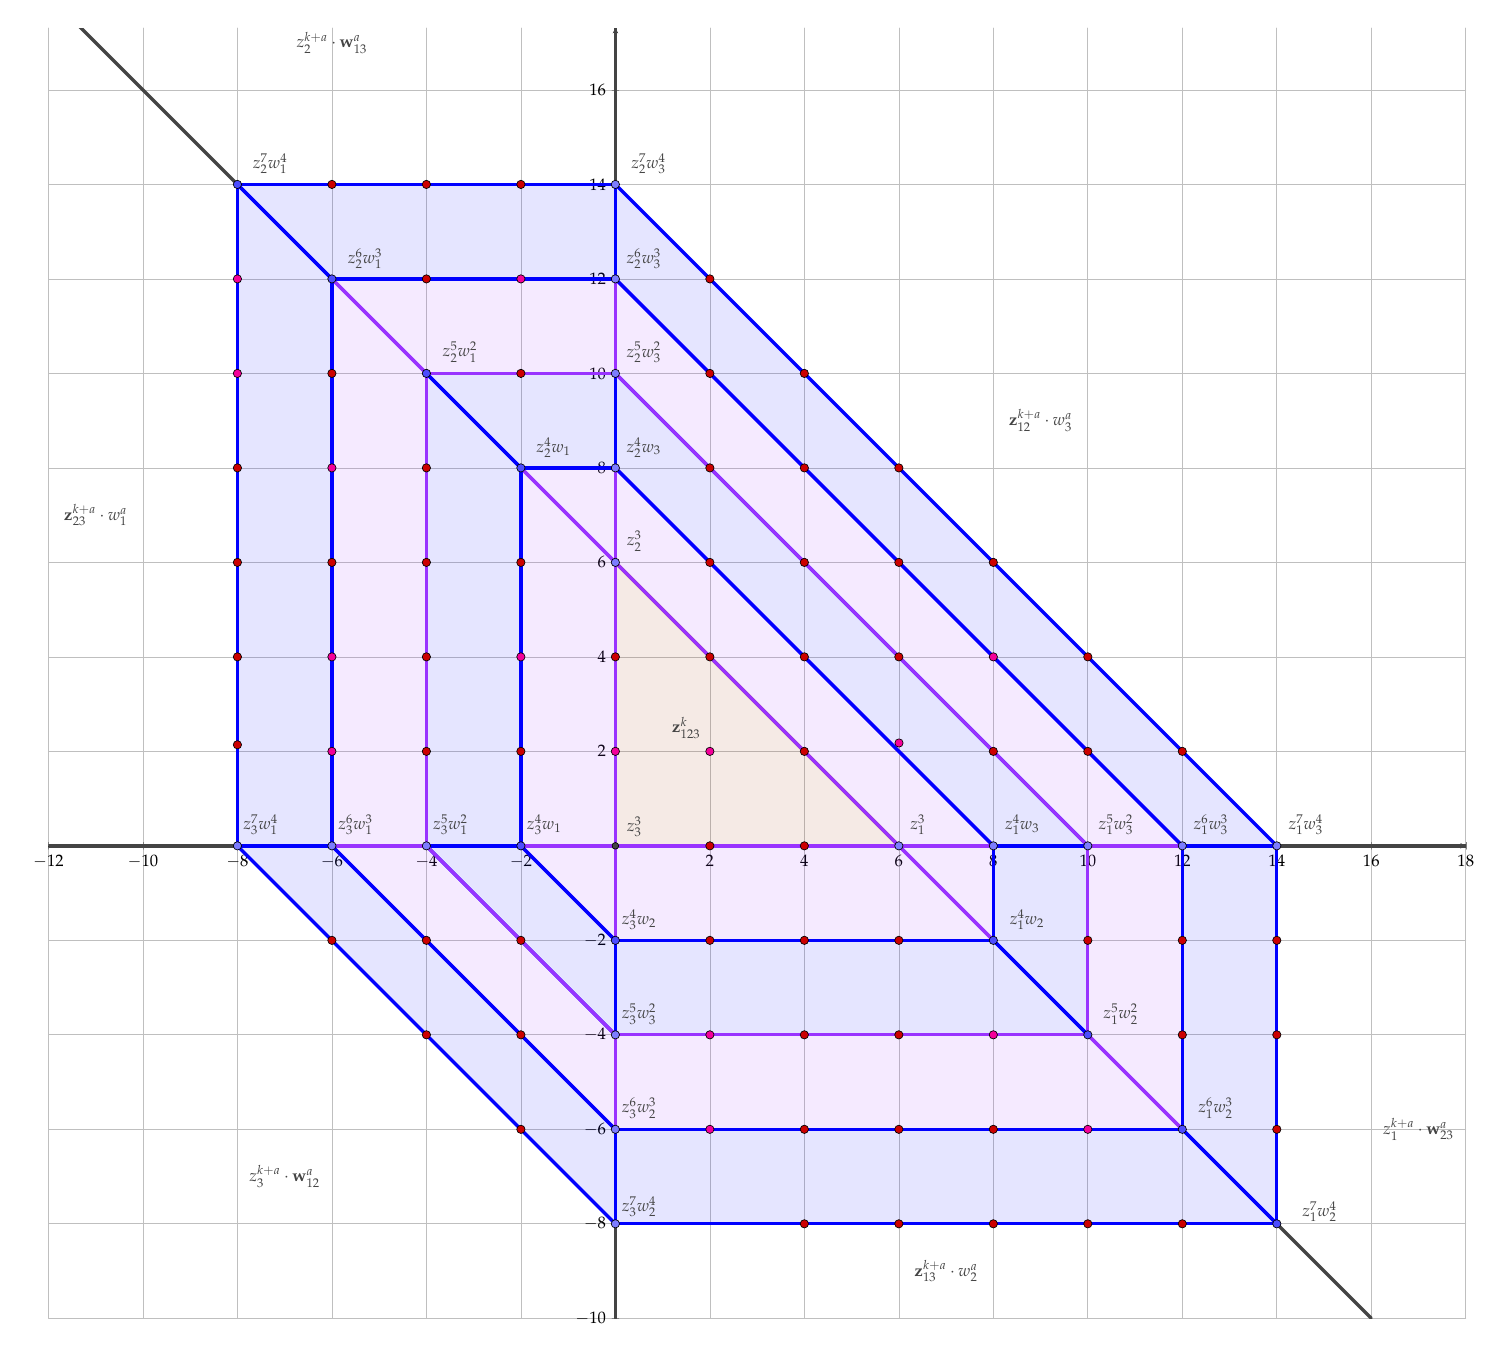
\begin{tikzpicture}[line cap=round,line join=round,>=triangle 45,x=1cm,y=1cm, scale=0.6]
	\begin{axis}[
		x=1cm,y=1cm,
		axis lines=middle,
		ymajorgrids=true,
		xmajorgrids=true,
		xmin=-12,
		xmax=18,
		ymin=-10,
		ymax=17.310846634374776,
		xtick={-12,-10,...,18},
		ytick={-10,-8,...,16},]
		%\clip(-17.075272789499802,-6.392711725783611) rectangle (24.908148373831658,17.310846634374776);
		\fill[line width=2pt,color=zzttqq,fill=zzttqq,fill opacity=0.10000000149011612] (0,6) -- (0,0) -- (6,0) -- cycle;
		\fill[line width=2pt,color=zzttff,fill=zzttff,fill opacity=0.1] (0,8) -- (0,6) -- (6,0) -- (8,0) -- cycle;
		\fill[line width=2pt,color=zzttff,fill=zzttff,fill opacity=0.1] (6,0) -- (8,-2) -- (0,-2) -- (0,0) -- cycle;
		\fill[line width=2pt,color=zzttff,fill=zzttff,fill opacity=0.1] (0,6) -- (-2,8) -- (-2,0) -- (0,0) -- cycle;
		\fill[line width=2pt,color=qqqqff,fill=qqqqff,fill opacity=0.1] (0,10) -- (10,0) -- (8,0) -- (0,8) -- cycle;
		\fill[line width=2pt,color=zzttff,fill=zzttff,fill opacity=0.1] (12,0) -- (10,0) -- (0,10) -- (0,12) -- cycle;
		\fill[line width=2pt,color=qqqqff,fill=qqqqff,fill opacity=0.1] (0,-2) -- (8,-2) -- (10,-4) -- (0,-4) -- cycle;
		\fill[line width=2pt,color=zzttff,fill=zzttff,fill opacity=0.1] (0,-6) -- (0,-4) -- (10,-4) -- (12,-6) -- cycle;
		\fill[line width=2pt,color=qqqqff,fill=qqqqff,fill opacity=0.1] (-2,8) -- (-4,10) -- (-4,0) -- (-2,0) -- cycle;
		\fill[line width=2pt,color=zzttff,fill=zzttff,fill opacity=0.1] (-6,12) -- (-4,10) -- (-4,0) -- (-6,0) -- cycle;
		\fill[line width=2pt,color=zzttff,fill=zzttff,fill opacity=0.1] (8,0) -- (8,-2) -- (6,0) -- cycle;
		\fill[line width=2pt,color=qqqqff,fill=qqqqff,fill opacity=0.1] (10,0) -- (8,0) -- (8,-2) -- (10,-4) -- cycle;
		\fill[line width=2pt,color=zzttff,fill=zzttff,fill opacity=0.1] (12,0) -- (10,0) -- (10,-4) -- (12,-6) -- cycle;
		\fill[line width=2pt,color=zzttff,fill=zzttff,fill opacity=0.1] (-2,0) -- (0,-2) -- (0,0) -- cycle;
		\fill[line width=2pt,color=qqqqff,fill=qqqqff,fill opacity=0.1] (-4,0) -- (0,-4) -- (0,-2) -- (-2,0) -- cycle;
		\fill[line width=2pt,color=zzttff,fill=zzttff,fill opacity=0.1] (-6,0) -- (0,-6) -- (0,-4) -- (-4,0) -- cycle;
		\fill[line width=2pt,color=zzttff,fill=zzttff,fill opacity=0.1] (0,8) -- (-2,8) -- (0,6) -- cycle;
		\fill[line width=2pt,color=qqqqff,fill=qqqqff,fill opacity=0.1] (-4,10) -- (0,10) -- (0,8) -- (-2,8) -- cycle;
		\fill[line width=2pt,color=zzttff,fill=zzttff,fill opacity=0.1] (-6,12) -- (0,12) -- (0,10) -- (-4,10) -- cycle;
		\fill[line width=2pt,color=qqqqff,fill=qqqqff,fill opacity=0.1] (0,14) -- (14,0) -- (12,0) -- (0,12) -- cycle;
		\fill[line width=2pt,color=qqqqff,fill=qqqqff,fill opacity=0.1] (-8,14) -- (-6,12) -- (0,12) -- (0,14) -- cycle;
		\fill[line width=2pt,color=qqqqff,fill=qqqqff,fill opacity=0.1] (-8,14) -- (-8,0) -- (-6,0) -- (-6,12) -- cycle;
		\fill[line width=2pt,color=qqqqff,fill=qqqqff,fill opacity=0.1] (-8,0) -- (0,-8) -- (0,-6) -- (-6,0) -- cycle;
		\fill[line width=2pt,color=qqqqff,fill=qqqqff,fill opacity=0.1] (14,-8) -- (0,-8) -- (0,-6) -- (12,-6) -- cycle;
		\fill[line width=2pt,color=qqqqff,fill=qqqqff,fill opacity=0.1] (14,0) -- (12,0) -- (12,-6) -- (14,-8) -- cycle;
		\draw [line width=2pt,color=zzttqq] (0,6)-- (0,0);
		\draw [line width=2pt,color=zzttqq] (0,0)-- (6,0);
		\draw [line width=2pt,color=zzttqq] (6,0)-- (0,6);
		\draw [line width=2pt,color=zzttff] (0,8)-- (0,6);
		\draw [line width=2pt,color=zzttff] (0,6)-- (6,0);
		\draw [line width=2pt,color=zzttff] (6,0)-- (8,0);
		\draw [line width=2pt,color=zzttff] (8,0)-- (0,8);
		\draw [line width=2pt,color=zzttff] (6,0)-- (8,-2);
		\draw [line width=2pt,color=zzttff] (8,-2)-- (0,-2);
		\draw [line width=2pt,color=zzttff] (0,-2)-- (0,0);
		\draw [line width=2pt,color=zzttff] (0,0)-- (6,0);
		\draw [line width=2pt,color=zzttff] (0,6)-- (-2,8);
		\draw [line width=2pt,color=zzttff] (-2,8)-- (-2,0);
		\draw [line width=2pt,color=zzttff] (-2,0)-- (0,0);
		\draw [line width=2pt,color=zzttff] (0,0)-- (0,6);
		\draw [line width=2pt,color=qqqqff] (0,10)-- (10,0);
		\draw [line width=2pt,color=qqqqff] (10,0)-- (8,0);
		\draw [line width=2pt,color=qqqqff] (8,0)-- (0,8);
		\draw [line width=2pt,color=qqqqff] (0,8)-- (0,10);
		\draw [line width=2pt,color=zzttff] (12,0)-- (10,0);
		\draw [line width=2pt,color=zzttff] (10,0)-- (0,10);
		\draw [line width=2pt,color=zzttff] (0,10)-- (0,12);
		\draw [line width=2pt,color=zzttff] (0,12)-- (12,0);
		\draw [line width=2pt,color=qqqqff] (0,-2)-- (8,-2);
		\draw [line width=2pt,color=qqqqff] (8,-2)-- (10,-4);
		\draw [line width=2pt,color=qqqqff] (10,-4)-- (0,-4);
		\draw [line width=2pt,color=qqqqff] (0,-4)-- (0,-2);
		\draw [line width=2pt,color=zzttff] (0,-6)-- (0,-4);
		\draw [line width=2pt,color=zzttff] (0,-4)-- (10,-4);
		\draw [line width=2pt,color=zzttff] (10,-4)-- (12,-6);
		\draw [line width=2pt,color=zzttff] (12,-6)-- (0,-6);
		\draw [line width=2pt,color=qqqqff] (-2,8)-- (-4,10);
		\draw [line width=2pt,color=qqqqff] (-4,10)-- (-4,0);
		\draw [line width=2pt,color=qqqqff] (-4,0)-- (-2,0);
		\draw [line width=2pt,color=qqqqff] (-2,0)-- (-2,8);
		\draw [line width=2pt,color=zzttff] (-6,12)-- (-4,10);
		\draw [line width=2pt,color=zzttff] (-4,10)-- (-4,0);
		\draw [line width=2pt,color=zzttff] (-4,0)-- (-6,0);
		\draw [line width=2pt,color=zzttff] (-6,0)-- (-6,12);
		\draw [line width=2pt,color=zzttff] (8,0)-- (8,-2);
		\draw [line width=2pt,color=zzttff] (8,-2)-- (6,0);
		\draw [line width=2pt,color=zzttff] (6,0)-- (8,0);
		\draw [line width=2pt,color=qqqqff] (10,0)-- (8,0);
		\draw [line width=2pt,color=qqqqff] (8,0)-- (8,-2);
		\draw [line width=2pt,color=qqqqff] (8,-2)-- (10,-4);
		\draw [line width=2pt,color=qqqqff] (10,-4)-- (10,0);
		\draw [line width=2pt,color=zzttff] (12,0)-- (10,0);
		\draw [line width=2pt,color=zzttff] (10,0)-- (10,-4);
		\draw [line width=2pt,color=zzttff] (10,-4)-- (12,-6);
		\draw [line width=2pt,color=zzttff] (12,-6)-- (12,0);
		\draw [line width=2pt,color=zzttff] (-2,0)-- (0,-2);
		\draw [line width=2pt,color=zzttff] (0,-2)-- (0,0);
		\draw [line width=2pt,color=zzttff] (0,0)-- (-2,0);
		\draw [line width=2pt,color=qqqqff] (-4,0)-- (0,-4);
		\draw [line width=2pt,color=qqqqff] (0,-4)-- (0,-2);
		\draw [line width=2pt,color=qqqqff] (0,-2)-- (-2,0);
		\draw [line width=2pt,color=qqqqff] (-2,0)-- (-4,0);
		\draw [line width=2pt,color=zzttff] (-6,0)-- (0,-6);
		\draw [line width=2pt,color=zzttff] (0,-6)-- (0,-4);
		\draw [line width=2pt,color=zzttff] (0,-4)-- (-4,0);
		\draw [line width=2pt,color=zzttff] (-4,0)-- (-6,0);
		\draw [line width=2pt,color=zzttff] (0,8)-- (-2,8);
		\draw [line width=2pt,color=zzttff] (-2,8)-- (0,6);
		\draw [line width=2pt,color=zzttff] (0,6)-- (0,8);
		\draw [line width=2pt,color=qqqqff] (-4,10)-- (0,10);
		\draw [line width=2pt,color=qqqqff] (0,10)-- (0,8);
		\draw [line width=2pt,color=qqqqff] (0,8)-- (-2,8);
		\draw [line width=2pt,color=qqqqff] (-2,8)-- (-4,10);
		\draw [line width=2pt,color=zzttff] (-6,12)-- (0,12);
		\draw [line width=2pt,color=zzttff] (0,12)-- (0,10);
		\draw [line width=2pt,color=zzttff] (0,10)-- (-4,10);
		\draw [line width=2pt,color=zzttff] (-4,10)-- (-6,12);
		\draw [line width=2pt,color=qqqqff] (0,14)-- (14,0);
		\draw [line width=2pt,color=qqqqff] (14,0)-- (12,0);
		\draw [line width=2pt,color=qqqqff] (12,0)-- (0,12);
		\draw [line width=2pt,color=qqqqff] (0,12)-- (0,14);
		\draw [line width=2pt,color=qqqqff] (-8,14)-- (-6,12);
		\draw [line width=2pt,color=qqqqff] (-6,12)-- (0,12);
		\draw [line width=2pt,color=qqqqff] (0,12)-- (0,14);
		\draw [line width=2pt,color=qqqqff] (0,14)-- (-8,14);
		\draw [line width=2pt,color=qqqqff] (-8,14)-- (-8,0);
		\draw [line width=2pt,color=qqqqff] (-8,0)-- (-6,0);
		\draw [line width=2pt,color=qqqqff] (-6,0)-- (-6,12);
		\draw [line width=2pt,color=qqqqff] (-6,12)-- (-8,14);
		\draw [line width=2pt,color=qqqqff] (-8,0)-- (0,-8);
		\draw [line width=2pt,color=qqqqff] (0,-8)-- (0,-6);
		\draw [line width=2pt,color=qqqqff] (0,-6)-- (-6,0);
		\draw [line width=2pt,color=qqqqff] (-6,0)-- (-8,0);
		\draw [line width=2pt,color=qqqqff] (14,-8)-- (0,-8);
		\draw [line width=2pt,color=qqqqff] (0,-8)-- (0,-6);
		\draw [line width=2pt,color=qqqqff] (0,-6)-- (12,-6);
		\draw [line width=2pt,color=qqqqff] (12,-6)-- (14,-8);
		\draw [line width=2pt,color=qqqqff] (14,0)-- (12,0);
		\draw [line width=2pt,color=qqqqff] (12,0)-- (12,-6);
		\draw [line width=2pt,color=qqqqff] (12,-6)-- (14,-8);
		\draw [line width=2pt,color=qqqqff] (14,-8)-- (14,0);
		
		\draw [line width=2pt,color=uuuuuu] (0,-8)-- (0,-10);
		\draw [line width=2pt,color=uuuuuu] (-8,0)-- (-12,0);
		
		\draw [line width=2pt,color=uuuuuu] (-8,14)-- (-12,18);
		\draw [line width=2pt,color=uuuuuu] (0,14)-- (0,18);
		
		\draw [line width=2pt,color=uuuuuu] (14,0)-- (18,0);
		\draw [line width=2pt,color=uuuuuu] (14,-8)-- (16,-10);
		
		\begin{scriptsize}
			
			% --------------------------------------------------------------------			
			
			% Bottom-left simplex:
			\draw [fill=uuuuuu] (0,0) circle (2pt);
			%\draw[color=uuuuuu] (0.6019571740081808,0.4999013778853264) node {$z_{3}^{3}$};
			\draw[color=uuuuuu] (0.4019571740081808,0.3999013778853264) node {$z_{3}^{3}$};
			\draw [fill=ududff] (0,-2) circle (2.5pt);
			\draw[color=uuuuuu] (0.5023959806190216,-1.558655351026066) node {$z_{3}^{4}w_{2}$};
			\draw [fill=xdxdff] (0,-4) circle (2.5pt);
			\draw[color=uuuuuu] (0.5023959806190216,-3.567431483242879) node {$z_{3}^{5}w_{3}^{2}$};
			\draw [fill=xdxdff] (0,-6) circle (2.5pt);
			\draw[color=uuuuuu] (0.5023959806190216,-5.551097913806981) node {$z_{3}^{6}w_{2}^{3}$};
			\draw [fill=xdxdff] (-8,0) circle (2.5pt);
			\draw[color=uuuuuu] (-7.507598846595534,0.4501207811907467) node {$z_{3}^{7}w_{1}^{4}$};
			\draw [fill=xdxdff] (0,-8) circle (2.5pt);
			\draw[color=uuuuuu] (0.5023959806190216,-7.642519923) node {$z_{3}^{7}w_{2}^{4}$};
			\draw [fill=xdxdff] (-4,0) circle (2.5pt);
			\draw[color=uuuuuu] (-3.4900465821619007,0.4501207811907467) node {$z_{3}^{5}w_{1}^{2}$};
			\draw [fill=ududff] (-2,0) circle (2.5pt);
			\draw[color=uuuuuu] (-1.5063801515977946,0.4501207811907467) node {$z_{3}^{4}w_{1}$};
			\draw [fill=xdxdff] (-6,0) circle (2.5pt);
			\draw[color=uuuuuu] (-5.498822714378717,0.4501207811907467) node {$z_{3}^{6}w_{1}^{3}$};
			
			% --------------------------------------------------------------------
			
			% Top-left simplex:
			\draw [fill=xdxdff] (0,6) circle (2.5pt);
			\draw[color=uuuuuu] (0.4019571740081808,6.451339476188474) node {$z_{2}^{3}$};

			\draw[color=uuuuuu] (0.6028347872298625,8.435005906752577) node {$z_{2}^{4}w_{3}$};
			\draw [fill=xdxdff] (8,0) circle (2.5pt);
			\draw [fill=ududff] (-2,8) circle (2.5pt);
			\draw[color=uuuuuu] (-1.305502538376113,8.435005906752577) node {$z_{2}^{4}w_{1}$};
			\draw [fill=xdxdff] (0,10) circle (2.5pt);
			\draw[color=uuuuuu] (0.6028347872298625,10.44378203896939) node {$z_{2}^{5}w_{3}^{2}$};
			\draw [fill=xdxdff] (10,0) circle (2.5pt);
	
			\draw[color=uuuuuu] (0.6028347872298625,12.427448469533493) node {$z_{2}^{6}w_{3}^{3}$};
			\draw [fill=ududff] (10,-4) circle (2.5pt);
			\draw [fill=xdxdff] (0,14) circle (2.5pt);
			\draw[color=uuuuuu] (0.7032735938407033,14.436224601750305) node {$z_{2}^{7}w_{3}^{4}$};
			\draw [fill=ududff] (-4,10) circle (2.5pt);
			\draw[color=uuuuuu] (-3.289168968940219,10.44378203896939) node {$z_{2}^{5}w_{1}^{2}$};
			\draw [fill=ududff] (-6,12) circle (2.5pt);
			\draw[color=uuuuuu] (-5.297945101157036,12.427448469533493) node {$z_{2}^{6}w_{1}^{3}$};
			\draw [fill=ududff] (-8,14) circle (2.5pt);
			\draw[color=uuuuuu] (-7.306721233373852,14.436224601750305) node {$z_{2}^{7}w_{1}^{4}$};
			
			% --------------------------------------------------------------------
			
			% Bottom-right simplex:
			\draw [fill=xdxdff] (6,0) circle (2.5pt);
			\draw[color=uuuuuu] (6.403175869005919,0.4501207811907467) node {$z_{1}^{3}$};
			\draw [fill=xdxdff] (0,8) circle (2.5pt);
			\draw[color=uuuuuu] (8.612829614444418,0.4501207811907467) node {$z_{1}^{4}w_{3}$};
			\draw [fill=ududff] (8,-2) circle (2.5pt);
			\draw[color=uuuuuu] (8.713268421055259,-1.558655351026066) node {$z_{1}^{4}w_{2}$};
			\draw[color=uuuuuu] (10.596496045008523,0.4501207811907467) node {$z_{1}^{5}w_{3}^{2}$};
			\draw [fill=xdxdff] (12,0) circle (2.5pt);
			\draw[color=uuuuuu] (12.605272177225339,0.4501207811907467) node {$z_{1}^{6}w_{3}^{3}$};
			\draw [fill=xdxdff] (0,12) circle (2.5pt);
			\draw[color=uuuuuu] (10.696934851619363,-3.567431483242879) node {$z_{1}^{5}w_{2}^{2}$};
			\draw [fill=ududff] (12,-6) circle (2.5pt);
			\draw[color=uuuuuu] (12.70571098383618,-5.551097913806981) node {$z_{1}^{6}w_{2}^{3}$};
			\draw [fill=xdxdff] (14,0) circle (2.5pt);
			\draw[color=uuuuuu] (14.614048309442155,0.4501207811907467) node {$z_{1}^{7}w_{3}^{4}$};
			
			\draw [fill=ududff] (14,-8) circle (2.5pt);
			\draw[color=uuuuuu] (14.90571098383618,-7.742519923) node {$z_{1}^{7}w_{2}^{4}$};
			
			% --------------------------------------------------------------------
			
			% General monomial for each component:
			
			\draw[color=uuuuuu] (1.5,2.5) node {$\mathbf{z}_{123}^{k}$}; % Delta123
			
			\draw[color=uuuuuu] (9,9) node {$\mathbf{z}_{12}^{k+a}\cdot w_{3}^{a}$}; % Delta 12
			
			\draw[color=uuuuuu] (-11,7) node {$\mathbf{z}_{23}^{k+a}\cdot w_{1}^{a}$}; % Delta 23

			\draw[color=uuuuuu] (7,-9) node {$\mathbf{z}_{13}^{k+a}\cdot w_{2}^{a}$}; % Delta 13

			\draw[color=uuuuuu] (17,-6) node {$z_{1}^{k+a} \cdot \mathbf{w}_{23}^{a}$}; % Delta 1
			
			\draw[color=uuuuuu] (-6,17) node {$z_{2}^{k+a} \cdot \mathbf{w}_{13}^{a}$}; % Delta 2
			
			\draw[color=uuuuuu] (-7,-7) node {$z_{3}^{k+a} \cdot \mathbf{w}_{12}^{a}$}; % Delta 3	
			
			% --------------------------------------------------------------------		
			
			\draw [fill=ccqqqq] (0,4) circle (2.5pt);
			\draw [fill=fuqqzz] (0,2) circle (2.5pt);
			\draw [fill=ccqqqq] (2,4) circle (2.5pt);
			\draw [fill=ccqqqq] (4,2) circle (2.5pt);
			\draw [fill=ccqqqq] (4,0) circle (2.5pt);
			\draw [fill=ccqqqq] (2,0) circle (2.5pt);
			\draw [fill=fuqqzz] (2,2) circle (2.5pt);
			\draw [fill=ccqqqq] (2,6) circle (2.5pt);
			\draw [fill=ccqqqq] (4,4) circle (2.5pt);
			\draw [fill=ccqqqq] (2,8) circle (2.5pt);
			\draw [fill=ccqqqq] (2,10) circle (2.5pt);
			\draw [fill=ccqqqq] (2,-2) circle (2.5pt);
			\draw [fill=fuqqzz] (2,-4) circle (2.5pt);
			\draw [fill=fuqqzz] (2,-6) circle (2.5pt);
			\draw [fill=ccqqqq] (4,-2) circle (2.5pt);
			\draw [fill=ccqqqq] (4,-4) circle (2.5pt);
			\draw [fill=ccqqqq] (4,-6) circle (2.5pt);
			\draw [fill=ccqqqq] (4,6) circle (2.5pt);
			\draw [fill=ccqqqq] (4,8) circle (2.5pt);
			\draw [fill=ccqqqq] (6,6) circle (2.5pt);
			\draw [fill=ccqqqq] (6,4) circle (2.5pt);
			\draw [fill=fuqqzz] (6.003383990076149,2.177572465261519) circle (2.5pt);
			\draw [fill=ccqqqq] (6,-2) circle (2.5pt);
			\draw [fill=ccqqqq] (6,-4) circle (2.5pt);
			\draw [fill=ccqqqq] (6,-6) circle (2.5pt);
			\draw [fill=fuqqzz] (8,-4) circle (2.5pt);
			\draw [fill=ccqqqq] (8,-6) circle (2.5pt);
			\draw [fill=ccqqqq] (8,2) circle (2.5pt);
			\draw [fill=fuqqzz] (8,4) circle (2.5pt);
			\draw [fill=ccqqqq] (8,6) circle (2.5pt);
			\draw [fill=ccqqqq] (6,8) circle (2.5pt);
			\draw [fill=ccqqqq] (4,10) circle (2.5pt);
			\draw [fill=ccqqqq] (10,4) circle (2.5pt);
			\draw [fill=ccqqqq] (10,2) circle (2.5pt);
			\draw [fill=ccqqqq] (10,-2) circle (2.5pt);
			\draw [fill=fuqqzz] (10,-6) circle (2.5pt);
			\draw [fill=ccqqqq] (-2,-6) circle (2.5pt);
			\draw [fill=ccqqqq] (-2,-4) circle (2.5pt);
			\draw [fill=ccqqqq] (-4,-4) circle (2.5pt);
			\draw [fill=ccqqqq] (-4,-2) circle (2.5pt);
			\draw [fill=ccqqqq] (-2,-2) circle (2.5pt);
			\draw [fill=ccqqqq] (-6,-2) circle (2.5pt);
			\draw [fill=fuqqzz] (-6,2) circle (2.5pt);
			\draw [fill=ccqqqq] (-4,2) circle (2.5pt);
			\draw [fill=ccqqqq] (-2,2) circle (2.5pt);
			\draw [fill=fuqqzz] (-2,4) circle (2.5pt);
			\draw [fill=ccqqqq] (-4,4) circle (2.5pt);
			\draw [fill=fuqqzz] (-6,4) circle (2.5pt);
			\draw [fill=ccqqqq] (-6,6) circle (2.5pt);
			\draw [fill=ccqqqq] (-4,6) circle (2.5pt);
			\draw [fill=ccqqqq] (-2,6) circle (2.5pt);
			\draw [fill=ccqqqq] (-4,8) circle (2.5pt);
			\draw [fill=fuqqzz] (-6,8) circle (2.5pt);
			\draw [fill=ccqqqq] (-6,10) circle (2.5pt);
			\draw [fill=ccqqqq] (-2,10) circle (2.5pt);
			\draw [fill=ccqqqq] (2,12) circle (2.5pt);
			\draw [fill=fuqqzz] (-2,12) circle (2.5pt);
			\draw [fill=ccqqqq] (-4,12) circle (2.5pt);
			\draw [fill=ccqqqq] (-2,14) circle (2.5pt);
			\draw [fill=ccqqqq] (-4,14) circle (2.5pt);
			\draw [fill=ccqqqq] (-6,14) circle (2.5pt);
			\draw [fill=fuqqzz] (-8,12) circle (2.5pt);
			\draw [fill=fuqqzz] (-8,10) circle (2.5pt);
			\draw [fill=ccqqqq] (-8,8) circle (2.5pt);
			\draw [fill=ccqqqq] (-8,6) circle (2.5pt);
			\draw [fill=ccqqqq] (-8,4) circle (2.5pt);
			\draw [fill=ccqqqq] (-8,2.1397356695619782) circle (2.5pt);
			\draw [fill=ccqqqq] (12,2) circle (2.5pt);
			\draw [fill=ccqqqq] (12,-2) circle (2.5pt);
			\draw [fill=ccqqqq] (14,-2) circle (2.5pt);
			\draw [fill=ccqqqq] (12,-4) circle (2.5pt);
			\draw [fill=ccqqqq] (14,-4) circle (2.5pt);
			\draw [fill=ccqqqq] (14,-6) circle (2.5pt);
			\draw [fill=ccqqqq] (10,-8) circle (2.5pt);
			\draw [fill=ccqqqq] (12,-8) circle (2.5pt);
			\draw [fill=ccqqqq] (8,-8) circle (2.5pt);
			\draw [fill=ccqqqq] (6,-8) circle (2.5pt);
			\draw [fill=ccqqqq] (4,-8) circle (2.5pt);
		\end{scriptsize}
	\end{axis}
\end{tikzpicture}

\begin{center}\rule{0.5\linewidth}{0.5pt}\end{center}

\hypertarget{calculations}{%
	\subsubsection{Calculations}\label{calculations}}

From the Jupyter notebook, we have:

\begin{table}[]
	\begin{tabular}{|l|l|l|l|}
		\hline
			     &                &                      &                \\
		$(k,a)$  & Cut Difference & $\#(\mathbb{Z}^{2} \cap \mathcal{P})$ & $\chi(M_{\leq a}; \mathcal{L}_{\leq a}^{k})$ \\
			     &                &                      &                \\ \hline
			     &                &                      &                \\	     
		$(k,0)$  & $\displaystyle \frac{\left(k + 1\right) \left(k + 2\right)}{2}$               & $\displaystyle \frac{\left(k + 1\right) \left(k + 2\right)}{2}$                     &                \\
			     &                &                      &                \\ \hline
			     &                &                      &                \\	     
		$(k,1)$  & $\displaystyle \left(k + 2\right) \left(k + 4\right)$               & $\displaystyle \frac{k^{2}}{2} + \frac{9 k}{2} + 7$                     &                \\
			     &                &                      &                \\ \hline
			     &                &                      &                \\	     
	    $(k,2)$  & $\displaystyle \frac{3 \left(k + 3\right) \left(k + 6\right)}{2}$               & $\displaystyle \frac{k^{2}}{2} + \frac{15 k}{2} + 19$                     &                \\
			     &                &                      &                \\ \hline
			     &                &                      &                \\	     
	    $(k,3)$  & $\displaystyle 2 \left(k + 4\right) \left(k + 8\right)$               & $\displaystyle \frac{k^{2}}{2} + \frac{21 k}{2} + 37$                     &                \\
			     &                &                      &                \\ \hline
			     &                &                      &                \\	     
		$(k,4)$  & $\displaystyle \frac{5 \left(k + 5\right) \left(k + 10\right)}{2}$               & $\displaystyle \frac{k^{2}}{2} + \frac{27 k}{2} + 61$                     &                \\
				 &                &                      &                \\ \hline
				 &                &                      &                \\	     
		$(k,5)$  & $\displaystyle 3 \left(k + 6\right) \left(k + 12\right)$               & $\displaystyle \frac{k^{2}}{2} + \frac{33 k}{2} + 91$                     &                \\
				 &                &                      &                \\ \hline
				 &                &                      &                \\	     
		$(k,6)$  & $\displaystyle \frac{7 \left(k + 7\right) \left(k + 14\right)}{2}$               & $\displaystyle \frac{k^{2}}{2} + \frac{39 k}{2} + 127$                     &                \\
				 &                &                      &                \\ \hline
				 &                &                      &                \\	     
		$(k,7)$  & $\displaystyle 4 \left(k + 8\right) \left(k + 16\right)$               & $\displaystyle \frac{k^{2}}{2} + \frac{45 k}{2} + 169$                     &                \\
				 &                &                      &                \\ \hline
				 &                &                      &                \\	     
		$(k,8)$  & $\displaystyle \frac{9 \left(k + 9\right) \left(k + 18\right)}{2}$               & $\displaystyle \frac{k^{2}}{2} + \frac{51 k}{2} + 217$                     &                \\
				 &                &                      &                \\ \hline
				 &                &                      &                \\	     
		$(k,9)$  & $\displaystyle 5 \left(k + 10\right) \left(k + 20\right)$               & $\displaystyle \frac{k^{2}}{2} + \frac{57 k}{2} + 271$                     &                \\
				 &                &                      &                \\ \hline
				 &                &                      &                \\	     
		$(k,10)$ &                &                      &                \\
				 &                &                      &                \\ \hline
	\end{tabular}
\end{table}

\newpage
 
\hypertarget{minkowski}{%
	\subsubsection{Minkowski Sum}\label{minkowski}}

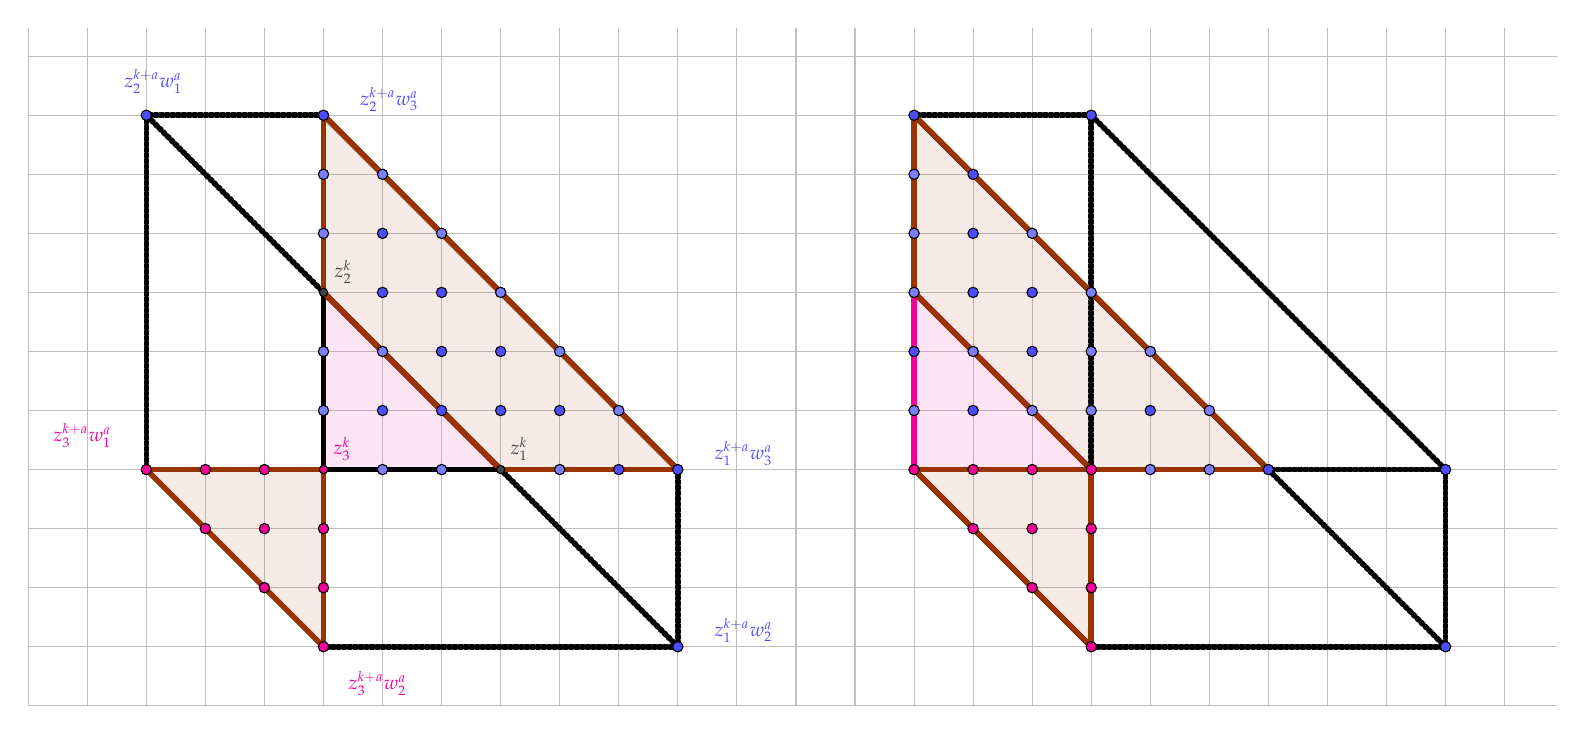
\begin{tikzpicture}[line cap=round,line join=round,>=triangle 45,x=1cm,y=1cm, scale=0.75]
	\draw [color=cqcqcq,, xstep=1cm,ystep=1cm] (-5,-4) grid (20.88371075992751,7.473463425890853);
	\clip(-5,-4) rectangle (20.88371075992751,7.473463425890853);
	\fill[line width=2pt,color=fuqqzz,fill=fuqqzz,fill opacity=0.1] (0,3) -- (3,0) -- (0,0) -- cycle;
	\fill[line width=2pt,color=zzttqq,fill=zzttqq,fill opacity=0.10000000149011612] (-3,0) -- (0,0) -- (0,-3) -- cycle;
	\fill[line width=2pt,color=zzttqq,fill=zzttqq,fill opacity=0.10000000149011612] (0,6) -- (0,3) -- (3,0) -- (6,0) -- cycle;
	\fill[line width=2pt,color=fuqqzz,fill=fuqqzz,fill opacity=0.1] (10,3) -- (13,0) -- (10,0) -- cycle;
	\fill[line width=2pt,color=zzttqq,fill=zzttqq,fill opacity=0.10000000149011612] (10,6) -- (16,0) -- (13,0) -- (10,3) -- cycle;
	\fill[line width=2pt,color=zzttqq,fill=zzttqq,fill opacity=0.10000000149011612] (10,0) -- (13,0) -- (13,-3) -- cycle;
	\draw [line width=2pt,color=fuqqzz] (0,3)-- (3,0);
	\draw [line width=2pt,color=fuqqzz] (3,0)-- (0,0);
	\draw [line width=2pt,color=fuqqzz] (0,0)-- (0,3);
	\draw [line width=2pt,dash pattern=on 1pt off 1pt] (6,-3)-- (-3,6);
	\draw [line width=2pt] (-3,0)-- (6,0);
	\draw [line width=2pt] (0,6)-- (0,-3);
	\draw [line width=2pt,color=zzttqq] (-3,0)-- (0,0);
	\draw [line width=2pt,color=zzttqq] (0,0)-- (0,-3);
	\draw [line width=2pt,color=zzttqq] (0,-3)-- (-3,0);
	\draw [line width=2pt,dash pattern=on 1pt off 1pt] (-3,6)-- (-3,0);
	\draw [line width=2pt,dash pattern=on 1pt off 1pt] (0,6)-- (-3,6);
	\draw [line width=2pt,dash pattern=on 1pt off 1pt] (6,-3)-- (0,-3);
	\draw [line width=2pt,dash pattern=on 1pt off 1pt] (6,0)-- (6,-3);
	\draw [line width=2pt] (6,0)-- (0,6);
	\draw [line width=2pt,color=zzttqq] (0,6)-- (0,3);
	\draw [line width=2pt,color=zzttqq] (0,3)-- (3,0);
	\draw [line width=2pt,color=zzttqq] (3,0)-- (6,0);
	\draw [line width=2pt,color=zzttqq] (6,0)-- (0,6);
	\draw [line width=2pt] (10,6)-- (10,0);
	\draw [line width=2pt] (10,0)-- (13,-3);
	\draw [line width=2pt] (13,-3)-- (13,0);
	\draw [line width=2pt] (10,0)-- (13,0);
	\draw [line width=2pt,color=fuqqzz] (10,3)-- (13,0);
	\draw [line width=2pt,color=fuqqzz] (13,0)-- (10,0);
	\draw [line width=2pt,color=fuqqzz] (10,0)-- (10,3);
	\draw [line width=2pt] (10,6)-- (16,0);
	\draw [line width=2pt] (13,0)-- (16,0);
	\draw [line width=2pt,dash pattern=on 1pt off 1pt] (16,0)-- (19,-3);
	\draw [line width=2pt,dash pattern=on 1pt off 1pt] (13,-3)-- (19,-3);
	\draw [line width=2pt,dash pattern=on 1pt off 1pt] (13,6)-- (10,6);
	\draw [line width=2pt,dash pattern=on 1pt off 1pt] (13,6)-- (13,3);
	\draw [line width=2pt,dash pattern=on 1pt off 1pt] (13,0)-- (13,3);
	\draw [line width=2pt,color=zzttqq] (10,6)-- (16,0);
	\draw [line width=2pt,color=zzttqq] (16,0)-- (13,0);
	\draw [line width=2pt,color=zzttqq] (13,0)-- (10,3);
	\draw [line width=2pt,color=zzttqq] (10,3)-- (10,6);
	\draw [line width=2pt,color=zzttqq] (10,0)-- (13,0);
	\draw [line width=2pt,color=zzttqq] (13,0)-- (13,-3);
	\draw [line width=2pt,color=zzttqq] (13,-3)-- (10,0);
	\draw [line width=2pt,dash pattern=on 1pt off 1pt] (19,0)-- (19,-3);
	\draw [line width=2pt,dash pattern=on 1pt off 1pt] (19,0)-- (16,0);
	\draw [line width=2pt,dash pattern=on 1pt off 1pt] (19,0)-- (13,6);
	\begin{scriptsize}
		\draw [fill=ududff] (6,-3) circle (2.5pt);
		\draw[color=ududff] (7.114044854739787,-2.72339333214169) node {$z_{1}^{k+a}w_{2}^{a}$};
		\draw [fill=ududff] (-3,6) circle (2.5pt);
		\draw[color=ududff] (-2.881644011026107,6.569712065948223) node {$z_{2}^{k+a}w_{1}^{a}$};
		\draw [fill=fuqqzz] (-3,0) circle (2.5pt);
		\draw[color=fuqqzz] (-4.081644011026107,0.5700624306786071) node {$z_{3}^{k+a}w_{1}^{a}$};
		\draw [fill=ududff] (6,0) circle (2.5pt);
		\draw[color=ududff] (7.114044854739787,0.2700624306786071) node {$z_{1}^{k+a}w_{3}^{a}$};
		\draw [fill=ududff] (0,6) circle (2.5pt);
		\draw[color=ududff] (1.11691894422919114,6.269712065948223) node {$z_{2}^{k+a}w_{3}^{a}$};
		\draw [fill=fuqqzz] (0,-3) circle (2.5pt);
		\draw[color=fuqqzz] (0.91691894422919114,-3.62339333214169) node {$z_{3}^{k+a}w_{2}^{a}$};
		\draw [fill=fuqqzz] (0,0) circle (2pt);
		\draw[color=fuqqzz] (0.31691894422919114,0.34458621142056197) node {$z_{3}^{k}$};
		\draw [fill=uuuuuu] (0,3) circle (2pt);
		\draw[color=uuuuuu] (0.33691894422919114,3.3507800838698815) node {$z_{2}^{k}$};
		\draw [fill=uuuuuu] (3,0) circle (2pt);
		\draw[color=uuuuuu] (3.315481899484489,0.34458621142056197) node {$z_{1}^{k}$};
		\draw [fill=ududff] (10,6) circle (2.5pt);
		\draw [fill=fuqqzz] (10,0) circle (2.5pt);
		\draw [fill=fuqqzz] (13,-3) circle (2.5pt);
		\draw [fill=fuqqzz] (13,0) circle (2.5pt);
		\draw [fill=xdxdff] (10,3) circle (2.5pt);
		\draw [fill=ududff] (16,0) circle (2.5pt);
		\draw [fill=ududff] (19,-3) circle (2.5pt);
		\draw [fill=ududff] (13,6) circle (2.5pt);
		\draw [fill=xdxdff] (13,3) circle (2.5pt);
		\draw [fill=ududff] (19,0) circle (2.5pt);
		\draw [fill=xdxdff] (0,1) circle (2.5pt);
		\draw [fill=xdxdff] (0,2) circle (2.5pt);
		\draw [fill=xdxdff] (0,4) circle (2.5pt);
		\draw [fill=xdxdff] (0,5) circle (2.5pt);
		\draw [fill=xdxdff] (1,5) circle (2.5pt);
		\draw [fill=ududff] (1,4) circle (2.5pt);
		\draw [fill=ududff] (1,3) circle (2.5pt);
		\draw [fill=xdxdff] (1,2) circle (2.5pt);
		\draw [fill=ududff] (1,1) circle (2.5pt);
		\draw [fill=xdxdff] (1,0) circle (2.5pt);
		\draw [fill=xdxdff] (2,0) circle (2.5pt);
		\draw [fill=ududff] (2,1) circle (2.5pt);
		\draw [fill=ududff] (2,2) circle (2.5pt);
		\draw [fill=ududff] (2,3) circle (2.5pt);
		\draw [fill=xdxdff] (2,4) circle (2.5pt);
		\draw [fill=xdxdff] (3,3) circle (2.5pt);
		\draw [fill=ududff] (3,2) circle (2.5pt);
		\draw [fill=ududff] (3,1) circle (2.5pt);
		\draw [fill=xdxdff] (4,0) circle (2.5pt);
		\draw [fill=ududff] (4,1) circle (2.5pt);
		\draw [fill=xdxdff] (4,2) circle (2.5pt);
		\draw [fill=xdxdff] (5,1) circle (2.5pt);
		\draw [fill=ududff] (5,0) circle (2.5pt);
		\draw [fill=fuqqzz] (-2,0) circle (2.5pt);
		\draw [fill=fuqqzz] (-2,-1) circle (2.5pt);
		\draw [fill=fuqqzz] (-1,-1) circle (2.5pt);
		\draw [fill=fuqqzz] (-1,0) circle (2.5pt);
		\draw [fill=fuqqzz] (0,-1) circle (2.5pt);
		\draw [fill=fuqqzz] (0,-2) circle (2.5pt);
		\draw [fill=fuqqzz] (-1,-2) circle (2.5pt);
		\draw [fill=xdxdff] (10,5) circle (2.5pt);
		\draw [fill=ududff] (11,5) circle (2.5pt);
		\draw [fill=xdxdff] (10,4) circle (2.5pt);
		\draw [fill=ududff] (11,4) circle (2.5pt);
		\draw [fill=xdxdff] (12,4) circle (2.5pt);
		\draw [fill=ududff] (11,3) circle (2.5pt);
		\draw [fill=ududff] (12,3) circle (2.5pt);
		\draw [fill=xdxdff] (14,2) circle (2.5pt);
		\draw [fill=xdxdff] (13,2) circle (2.5pt);
		\draw [fill=ududff] (12,2) circle (2.5pt);
		\draw [fill=xdxdff] (11,2) circle (2.5pt);
		\draw [fill=ududff] (10,2) circle (2.5pt);
		\draw [fill=xdxdff] (10,1) circle (2.5pt);
		\draw [fill=ududff] (11,1) circle (2.5pt);
		\draw [fill=xdxdff] (12,1) circle (2.5pt);
		\draw [fill=xdxdff] (13,1) circle (2.5pt);
		\draw [fill=ududff] (14,1) circle (2.5pt);
		\draw [fill=xdxdff] (15,1) circle (2.5pt);
		\draw [fill=xdxdff] (15,0) circle (2.5pt);
		\draw [fill=xdxdff] (14,0) circle (2.5pt);
		\draw [fill=fuqqzz] (12,0) circle (2.5pt);
		\draw [fill=fuqqzz] (11,0) circle (2.5pt);
		\draw [fill=fuqqzz] (11,-1) circle (2.5pt);
		\draw [fill=fuqqzz] (12,-1) circle (2.5pt);
		\draw [fill=fuqqzz] (13,-1) circle (2.5pt);
		\draw [fill=fuqqzz] (13,-2) circle (2.5pt);
		\draw [fill=fuqqzz] (12,-2) circle (2.5pt);
	\end{scriptsize}
\end{tikzpicture}
 
 \begin{equation*}
 	\begin{split}
 		H^{0}\left(\mathbb{CP}^{2}; \mathcal{O}(a)\right) \cong \mathbb{C}[&w_{1}^{a_{1}}w_{2}^{a_{2}}w_{3}^{a_{3}} : a_{1} + a_{2} + a_{3} = a] \\
 		= \mathbb{C}[&w_{1}^{a}, w_{1}^{a-1}w_{2}, \ldots, w_{1}w_{2}^{a-1}, w_{2}^{a} \, | \\
 		&w_{1}^{a-1}w_{3}, w_{1}^{a-2}w_{3}^{2}, \ldots w_{1}w_{3}^{a-1}, w_{3}^{a} \, | \\
 		&w_{2}^{a-1}w_{3}, w_{2}^{a-2}w_{3}^{2}, \ldots, w_{2}^{a}w_{3}^{a-2}, w_{2}w_{3}^{a-1} \, | \\
 		&w_{1}^{a-2}w_{2}w_{3}, w_{1}^{a-3}w_{2}^{2}w_{3}, \ldots, w_{1}w_{2}^{2}w_{3}^{a-3}, w_{1}w_{2}^{2}w_{3}^{a-2}].
 	\end{split}
 \end{equation*}

Examples: $a = 1, 2, 3$:
 
 \begin{equation*}
 	\begin{split}
 		H^{0}\left(\mathbb{CP}^{2}; \mathcal{O}(1)\right) &= \mathbb{C}[w_{1}, w_{2}, w_{3}], \\
 		H^{0}\left(\mathbb{CP}^{2}; \mathcal{O}(2)\right) &= \mathbb{C}[w_{1}^{2}, w_{1}w_{2}, w_{2}^{2} \, | w_{1}w_{3}, w_{3}^{2} \, | w_{2}w_{3} ], \\
 		H^{0}\left(\mathbb{CP}^{2}; \mathcal{O}(3)\right) &= \mathbb{C}[w_{1}^{3}, w_{1}^{2}w_{2}, w_{1}w_{2}^{2}, w_{2}^{3}\, | \, w_{1}^{2}w_{3}, w_{1}w_{3}^{2}, w_{3}^{3} \, | \,  w_{2}^{2}w_{3}, w_{2}w_{3}^{2}  \, | \, w_{1}w_{2}w_{3}]. 	 		
 	\end{split}
 \end{equation*}
 
The number of monomials equals:
\begin{equation*}
	h^{0}(\mathbb{CP}^{2}; \mathcal{O}(a)) = \frac{(a+1)(a+2)}{2}.
\end{equation*}
 
 
 
 
 
 
 
 
 
 















    % Add a bibliography block to the postdoc
    
    
    
\end{document}
